%
% Unless otherwise indicated, the copyright in this material is 
% owned by Joerg Evermann. This material is licensed to you under the 
% Creative Commons by-attribution non-commercial license (CC BY-NC 4.0)}
%

\section{Introduction}

Business process analytics is concerned with using event data to improve the \emph{operational efficiencies} of business processes. A business process is how an organization creates value for its customers. Improvements to operations may yield better customer service and increase customer satisfaction, it may also reduce the time it takes to complete a business process, it may reduce employee workload and improve employee satisfaction, it may reduce cost, or free up capacity. 

Every organization manages and executed a multitude of business processes. An important business process in many organizations is the order-to-cash process, which is the sequence of activities that begins when a customer submits an order and ends when the money has been received and a receipt has been issued. Another important process is issue-to-resolution, which begins when a customer contacts the organization with a problem about a product or service, and ends when the problem has been resolved to the satisfaction of the customer. Business processes exist in all kinds of organizations, from for-profit manufacturing or service enterprises, to healthcare clinics and hospital, to education and government services, to non-profit and charity organizations. Typically, a business process is characterized by its \emph{business object}. For example, the business of for the order-to-cash process is the customer order, the business object for the issue-to-resolution process is the customer complaint.

\section{Business Processes and Business Process Models}

A business process\index{Business process} is defined as a \emph{sequence of activities} that are executed in a defined order to create some type of \emph{value for a customer}. Besides activities, a business process also includes the \emph{resources} that carry out activities. Resources may be human resources, that is people or employees, or they may be machines or computer systems. Resources typically play one or more \emph{roles} in organization, such as accountants, warehouse workers, service technician, etc.

A business process may also contain \emph{events}. Events can trigger or start a business process or they may occur within a business process. Typical events are customer orders arriving, customer inquiries arriving, goods or materials arriving, goods or materials being dispatched, etc. 

A business process may also contain \emph{decisions}. For example, in an order-to-cash process, a decision may need to be made how to source a part, or how to ship a part, or whether to invoice a customer, etc. In a healthcare process, decisions may involve treatment options, medical tests, or hospital admissions.

Business processes are typically defined using business process models or business process diagrams. A common way to describe processes is with the \emph{Business Process Modelling Notation (BPMN)}, the industry standard developed by the OMG (Object Management Group)\footnote{\url{https://www.omg.org/bpmn/}} and adopted as the ISO/IEC 19510 standard. Figure~\ref{fig:bpmn} shows an example of a business process model in BPMN.

\begin{figure}
\centering
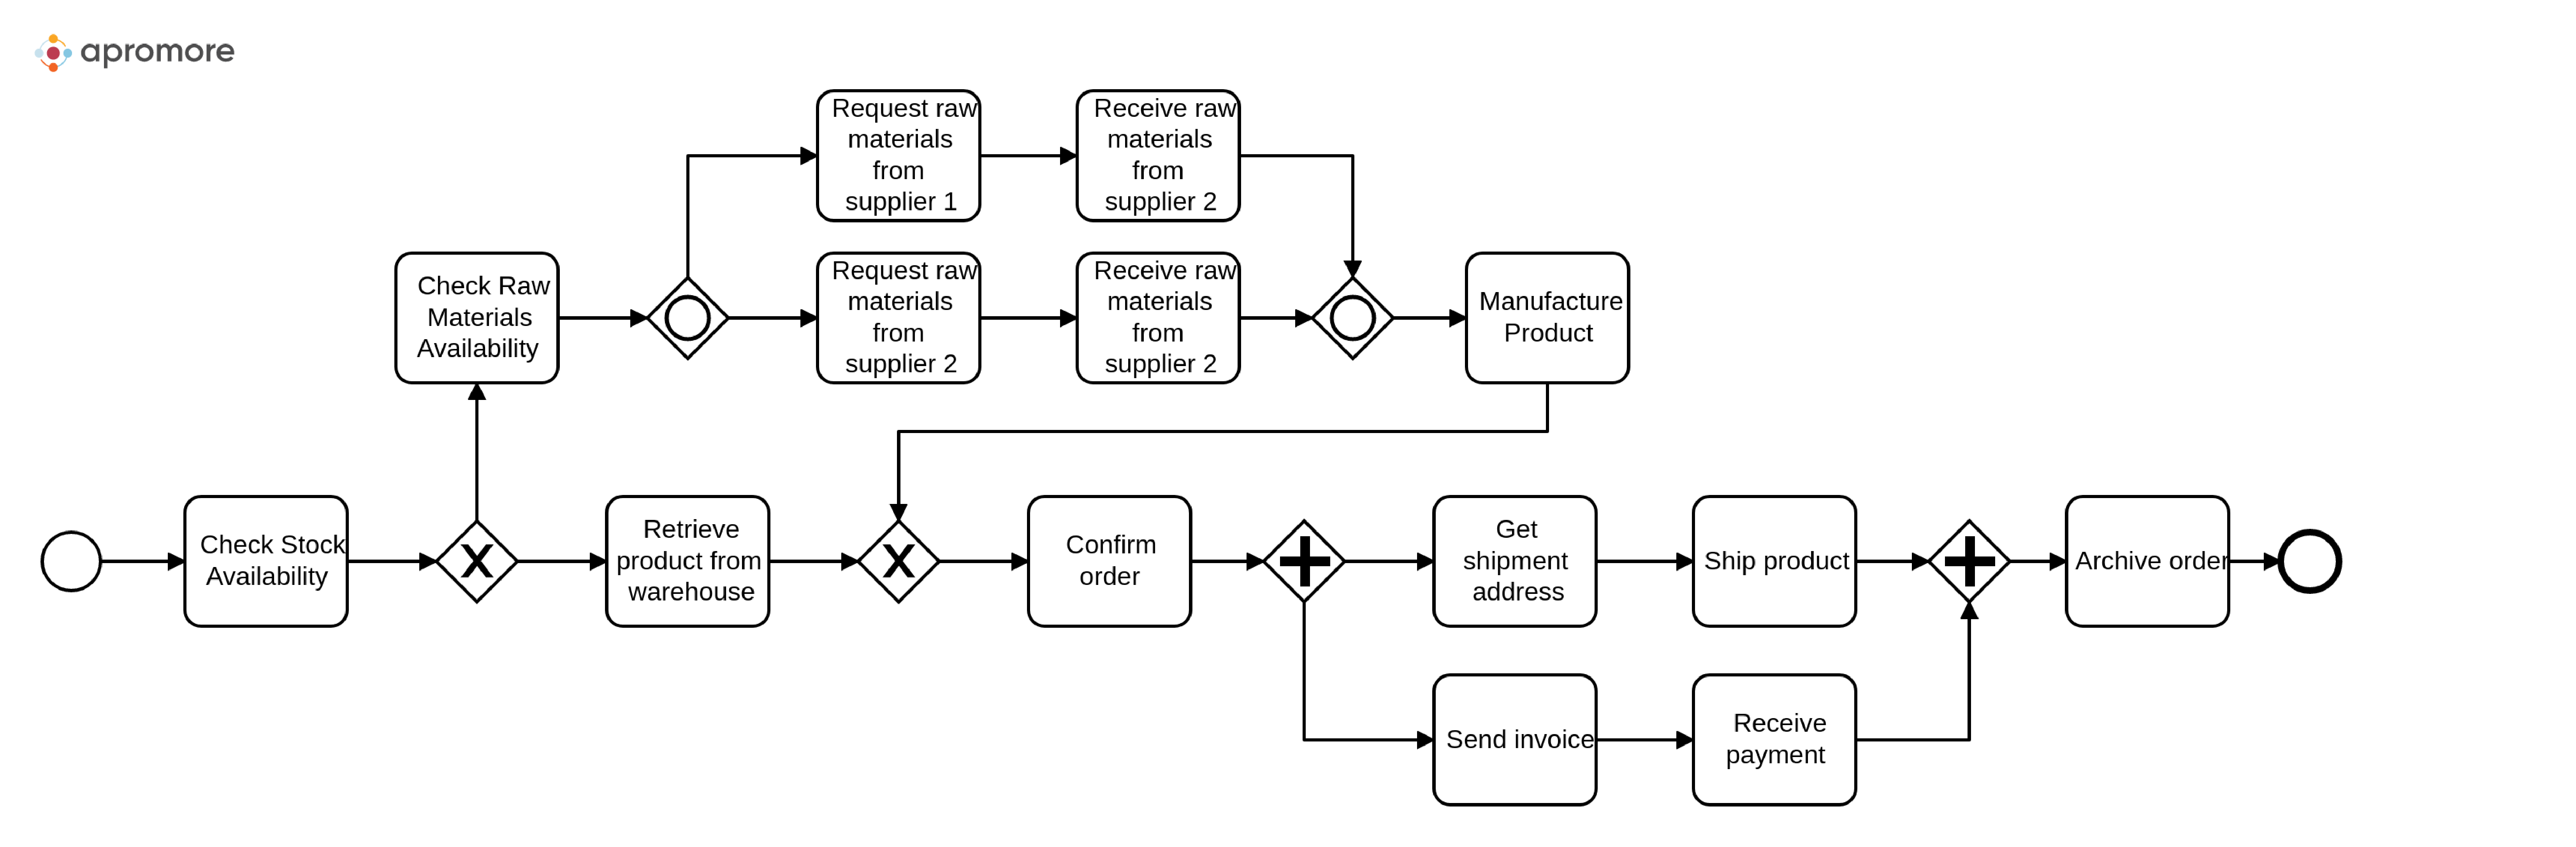
\includegraphics[width=1.1\textwidth]{Figure3.12.pdf} \\

\scriptsize Source: Marlon Dumas, Marcello La Rosa, Jan Mendling, Hajo A. Reijers (2018) ''Fundamentals of Business Process Management'', 2nd edition, Springer Verlag. Figure 3.12.
\caption{Example BPMN model}
\label{fig:bpmn}
\end{figure}

In this model, the circles represent events, rectangles represent activities, diamond shapes represent ''gateways'' and arrows represent process flow \emph{dependencies}. Dependencies describe what must happen before something else can happen, or, alternatively, what can follow once something is completed. 

The diamond with the ''$\times$'' symbol represents an \emph{exclusive gateway}, which means that a decision is made and only one outgoing path can be taken by the process. For example, after the activity ''Check Stock Availability'', either the activity ''Check Raw Materials Availability'' is carried out, or the ''Retrieve product from warehouse'' activity. 

In contrast, the ''$+$'' symbol represents a \emph{parallel gateway}, which means that the process proceeds along \emph{all} outgoing paths, in any order, or possibly at the same time. For example, after the ''Confirm order'' activity, both the ''Get shipment address'' and the ''Send invoice'' activities are carried out, in any order and possibly at the same time.

Finally, the ''$\bigcirc$'' symbol represents an \emph{inclusive gateway}. The process may proceed along any number of outgoing paths. For example, after the ''Check Raw Materials Availability'' activity, the process may proceed with the ''Request raw materials from supplier 1'' activity, or the ''Request raw materials from supplier 2'' activity, or both of them.

\section{Business Process Event Logs}

A \emph{case}\index{Case (of business process} is one instance of a business process. For example, the execution of the order-to-cash process and its activities for the order number 1234 is one case (instance); executing the process for order number 2345 is another case (instance). 

A \emph{trace}\index{Trace} is the sequence of events for one case. An \emph{event}\index{Event (of business process)} in this context is usually the execution of an activity instance (for example, ''Check Stock Availability'' for order 1234) or the occurrence of an outside event (for example, ''goods have arrived at warehouse''). However, activity instances themselves can have a complicated lifecycle. Figure~\ref{fig:activitylifecycle} shows an example of the lifecycle model of the XES standard\footnote{\url{https://www.tf-pm.org/resources/xes-standard}} for event log data. The XES standard defines how event data is represented in an XML document.

Each arrow in this figure represents a lifecycle transition and each box represents a lifecycle state. For example, an activity instance is first scheduled, then assigned to a resource, then started by the resources, and finally completed successfully. However, other lifecycles are possible in the XES lifecycle model. For example a resource may be repeatedly reassigned before being started, it may be suspended and resumed, and it may be skipped or aborted. Each of these lifecycle transitions may be captured by an \emph{event} in an event log.

\begin{figure}
\centering
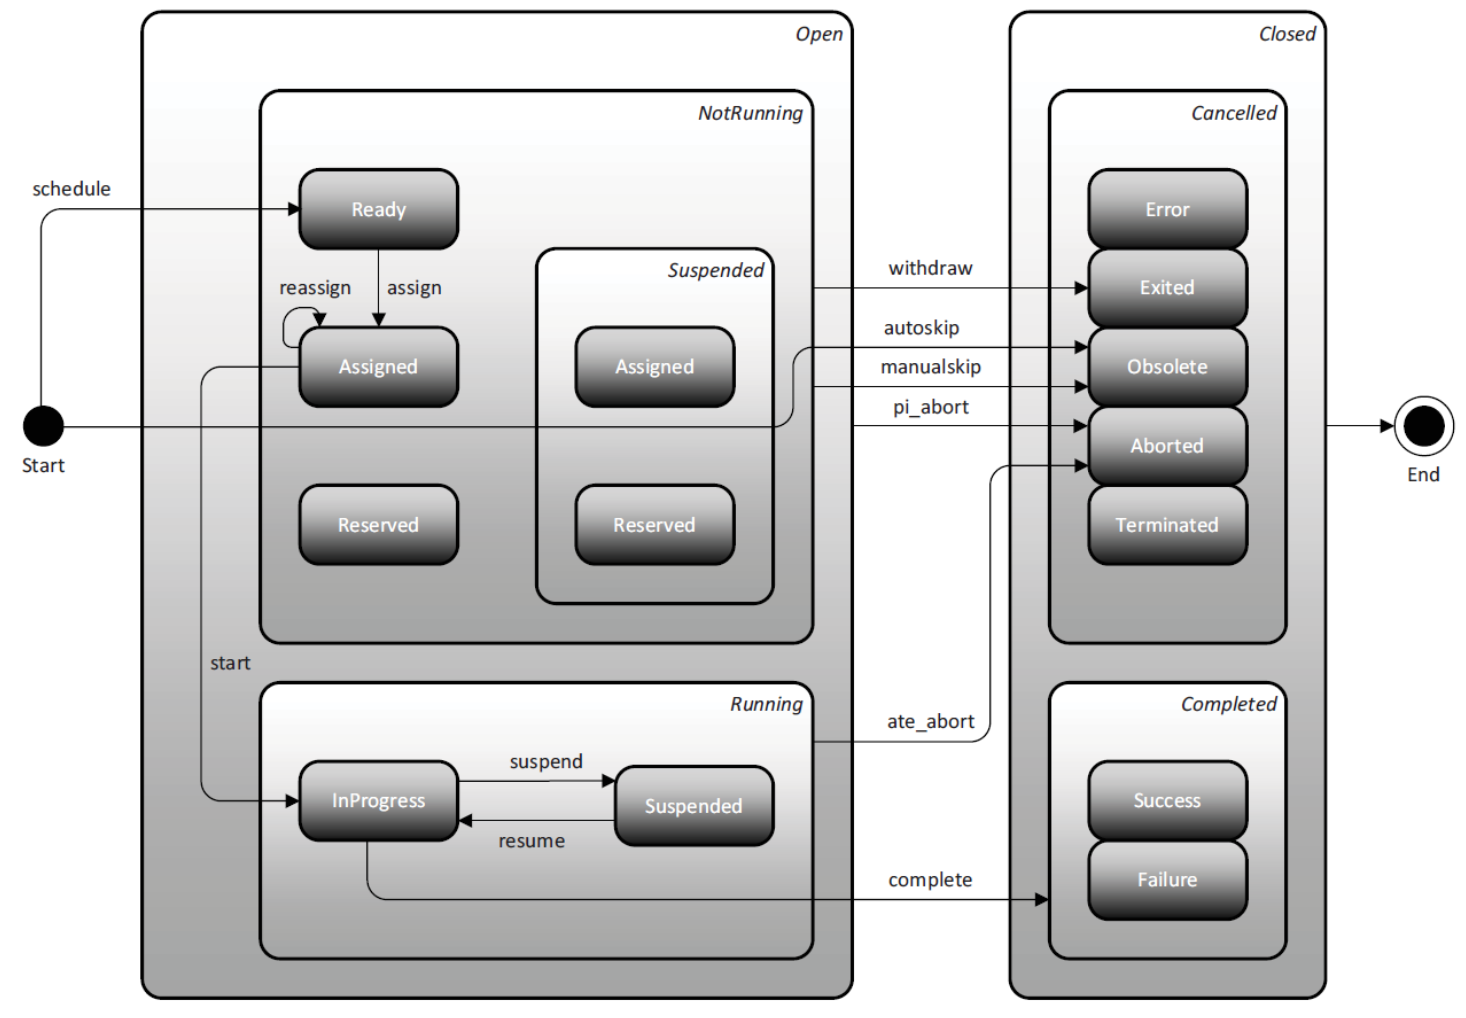
\includegraphics[height=2.5in]{screen1.png}

\scriptsize Source: \url{https://www.tf-pm.org/resources/xes-standard/about-xes/standard-extensions/lifecycle/standard}
\normalsize
\caption{Process Activity Lifecycle}
\label{fig:activitylifecycle}
\end{figure}

Each event may be associated with additional information, either about the particular activity instance or about the case. These are called \emph{event attributes} or \emph{case attributes}. Case attributes in an order-to-cash process instance may be name of the customer, the list of ordered products, etc. An example of an event attribute for a ''Confirm order'' activity instance completion event is the confirmation number that is generated by the activity instance. Each event is also typically associated with information about the resource that executed the activity instance that the event refers to, as well as a timestamp of when the event occurred.

An \emph{event log}\index{Event log} is a collection of one or more traces for one process. Hence, an event log describes the execution of one or more cases of the same process. Note that event logs may contain incomplete cases (e.g. cases that have not been completed when the event log was collected), may be randomly sampled from the complete event log data, etc.

Event logs are typically generated by process-aware information systems such as dedicated workflow-management systems, but many other corporate information systems, such as Enterprise Resource Planning (ERP) systems, Supply Chain Management (SCM) systems, Customer Relationship Management (CRM) systems, and other, keep track of \emph{who did what when}, which is the basic information in any event log. Additionally, event logs may be collected from any web-based information system as web-servers routinely keep log information about user interaction with the web site. 

To be usable for process analytics, the event log information from source information systems must typically be extracted, transformed and then loaded into a format that is used by process analytics software. This is known as an \emph{ETL process}: Extraction--Transformation--Load. ETL processes are required for many analytics applications that take their raw data from a variety of sources.

The standardized interchange format for event log data is the XES file format\index{Extensible event stream}\index{XES|see{Extensible event stream}}. XES stands for eXtensible Event Stream and is an XML based format. Another common format used for event log data are CSV files, where each row typically corresponds to one activity instance (not one event!). Below is an example of an XES file that uses the standard XES activity lifecycle model, defines three case attributes (''REG\_DATE'', ''AMOUNT\_REQ'', and ''concept:name'') and three event attributes (''time:timestamp'', ''lifecycle::transition'' and ''concept:name'' and then contains traces with their events. The XML code below is an excerpt of an XES file and illustrates how traces and events are encoded in XML.

\begin{xmlcode}
<?xml version="1.0" encoding="UTF-8" ?>
<log xes.version="1.0" xes.features="nested-attributes" 
    openxes.version="1.0RC7" 
    xmlns="http://www.xes-standard.org/">
  <extension name="Lifecycle" prefix="lifecycle" 
    uri="http://www.xes-standard.org/lifecycle.xesext"/>
  <extension name="Organizational" prefix="org" 
    uri="http://www.xes-standard.org/org.xesext"/>
  <extension name="Time" prefix="time" 
    uri="http://www.xes-standard.org/time.xesext"/>
  <extension name="Concept" prefix="concept" 
    uri="http://www.xes-standard.org/concept.xesext"/>
  <global scope="trace">
    <date key="REG_DATE" value="1970-01-01T00:00:00.000+01:00"/>
    <string key="AMOUNT_REQ" value="UNKNOWN"/>
    <string key="concept:name" value="UNKNOWN"/>
  </global>
  <global scope="event">
    <date key="time:timestamp" value="1970-01-01T00:00:00.000+01:00"/>
    <string key="lifecycle:transition" value="UNKNOWN"/>
    <string key="concept:name" value="UNKNOWN"/>
  </global>
  <classifier name="Activity classifier" 
     keys="concept:name lifecycle:transition"/>
  <classifier name="Resource classifier" 
     keys="org:resource"/>
  <trace>
    <date key="REG_DATE" value="2011-10-01T09:45:37.274+02:00"/>
    <string key="concept:name" value="173706"/>
    <string key="AMOUNT_REQ" value="18000"/>
    <event>
      <string key="org:resource" value="112"/>
      <string key="lifecycle:transition" value="COMPLETE"/>
      <string key="concept:name" value="A_SUBMITTED"/>
      <date key="time:timestamp" value="2011-10-01T09:45:37.274+02:00"/>
    </event>
    <event>
      <string key="org:resource" value="112"/>
      <string key="lifecycle:transition" value="COMPLETE"/>
      <string key="concept:name" value="A_PARTLYSUBMITTED"/>
      <date key="time:timestamp" value="2011-10-01T09:45:37.363+02:00"/>
    </event>
    ...
  </trace>
  ...
</log>
\end{xmlcode}

The file below is an excerpt of a CSV file that contains event log information (line breaks have been added to fit this into the width of the page but are not in the actual file). Note how ''Start Timestamp'' and ''Complete Timestamp'' exist for each row. This means that one row captures two events, the starting and the completion of an activity instance. 

\begin{textcode}
Case ID,Start Timestamp,Complete Timestamp,Activity,Resource,Role
339,2011/02/16 14:31:00.000,2011/02/16 15:23:00.000,
    Create Purchase Requisition,Nico Ojenbeer,Requester
339,2011/02/17 09:34:00.000,2011/02/17 09:40:00.000,
    Analyze Purchase Requisition,Maris Freeman,Requester Manager
339,2011/02/17 21:29:00.000,2011/02/17 21:52:00.000,
    Amend Purchase Requisition,Elvira Lores,Requester
339,2011/02/18 17:24:00.000,2011/02/18 17:30:00.000,
    Analyze Purchase Requisition,Heinz Gutschmidt,Requester Manager
\end{textcode}

\section{Types and Goals of Process Analytics}

The diagram in Figure~\ref{fig:processanalytics} shows four important activities in process analytics. Automated process discovery discovers a process model from an event log. This is useful to understand how a process is actually executed. The discovered process can then be analyzed for weaknesses or compared to a normative process model, e.g. as part of an audit. Many organizations also do not have well-defined processes, so that automated discovery is an important first step in understanding their own operations in detail.

\begin{figure}
\centering
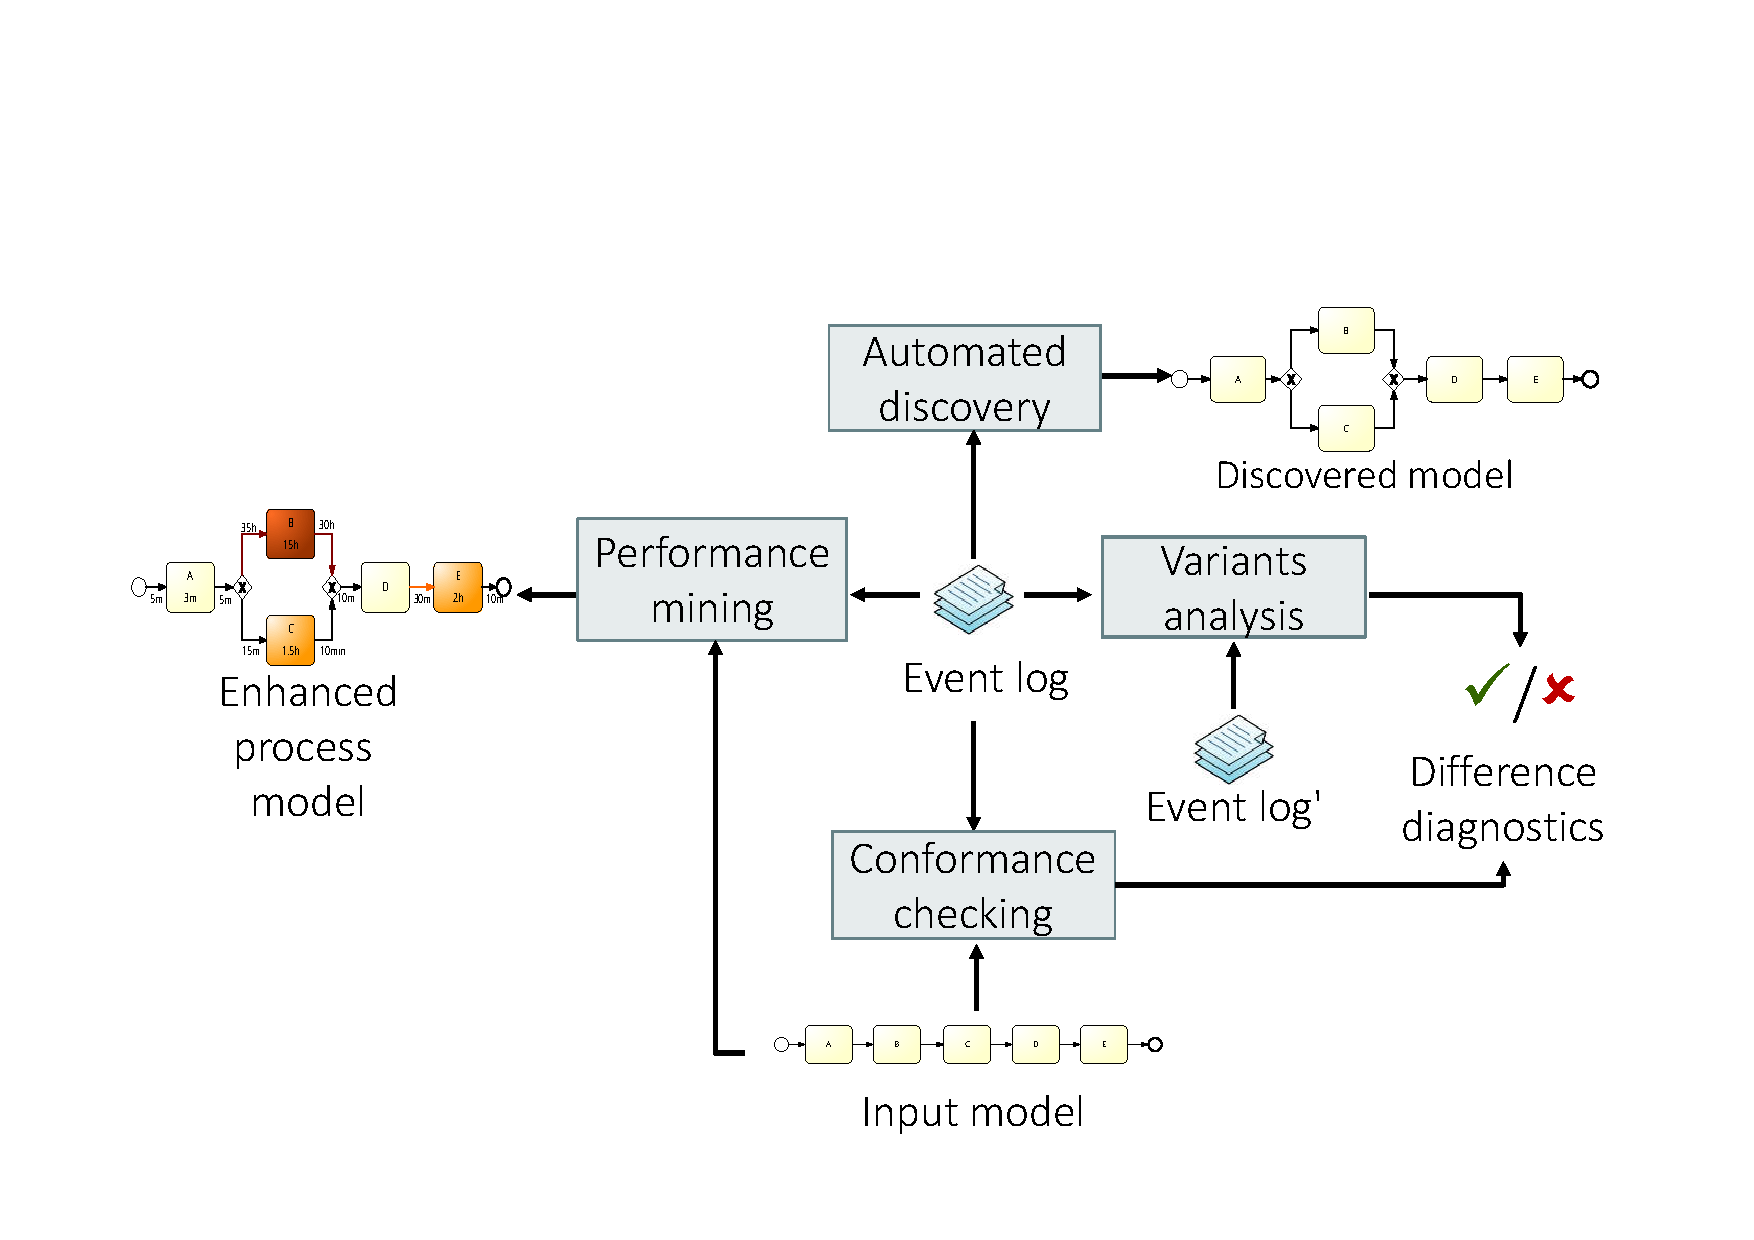
\includegraphics[width=.9\textwidth]{Chapter-11-Figure-03.pdf}\\
\vspace{3mm}\hrule\vspace{2mm}
\scriptsize{Source: Marlon Dumas, Marcello La Rosa, Jan Mendling, Hajo A. Reijers (2018) ''Fundamentals of Business Process Management'', 2nd edition, Springer Verlag. Figure 11.3}
\caption{Overview of Process Analytics with Event Logs}
\label{fig:processanalytics}
\end{figure}

Conformance checking compares an event log to a given input process model. It checks whether the actual operations, as captured in the event log, conform to or comply with a normative process model, a set of business rules, or a set of process constraints. This is typically done as part of an audit to demonstrate compliance, for example in the financial services industry, healthcare, or for quality management certifications. 

Performance mining enhances a process model (which could be an automatically discovered one) with information about the duration of activities and waiting times between activities, as captured in an event log. From there, process analysts can identify bottlenecks in the process, that is, activities where cases have to wait to be processed, activities that take a long time, activities with high variability in their processing time, or similar process problems. Further information can then be collected to identify the causes of and remedies for these problems.

Finally, variants analysis compares two different event logs of the same or similar processes to understand differences in execution. This may be useful when organizations execute the same business processes in different locations, or in different business units. This could be used to identify best practices for an organization.

In addition to these four, process prediction has become an important aspect of business process analytics. Process prediction uses an event log to train a statistical model in order to predict the future course or outcome of a currently running case. Typical prediction targets are the remaining time to completion of the case, the most likely next activity, the probability of a negative or positive outcome, the waiting time before the next activity starts, etc. Process prediction is useful to allow process managers to proactively intervene in a case before a problem arises, or before a case becomes late or overdue. Process prediction can also serve to provide information to customers about the how their case will likely be handled or completed.

Overall, the purposes of process analytics are multiple:
\begin{itemize}
   \item Discover actual operations
   \item Check actual process against desired process
   \item Identify operational (performance) problems
   \item Improve operational processes
   \item External compliance analysis and reporting
   \item Identify implicit or de-facto organizational groups and relationships 
   \item Support, reinforce, or break organizational relationships
\end{itemize}

\section{Process Analytics Tools}

Since the inception of the field of process analytics circa early 2000s, a range of commercial and open-source tools have been developed to support process analysts. Among the widely-used commercial tools are Celonis, Signavio, Fluxicon, ARIS and Apromore.

\paragraph*{Celonis}
Celonis\footnote{\url{https://www.celonis.com/}} is a leading process mining software that excels in helping organizations analyze and optimize their business processes through powerful data visualization and analytics. This tool extracts and leverages data from various IT systems to provide real-time insights into process performance, identify bottlenecks, and uncover inefficiencies. Celonis facilitates extensive process discovery, conformance checking, and predictive modeling, empowering users to drive significant improvements in process efficiency and effectiveness. Its capabilities are enhanced by features like machine learning and automation, making Celonis a pivotal tool for enterprises aiming to execute large-scale digital transformation strategies and achieve operational excellence.


\paragraph*{Signavio Process Manager}
Signavio\footnote{\url{https://www.signavio.com/}} Process Miner, part of the Signavio Business Transformation Suite, enables organizations to analyze and optimize business processes by visualizing actual workflows and identifying deviations from ideal models. This tool automatically generates process models from data logs, performs conformance checks to ensure regulatory compliance, and analyzes process performance metrics such as duration, frequency, and costs. Its integration with Signavio's broader suite allows for a seamless workflow from process discovery through modeling to execution, making it a valuable tool for continuous process improvement and alignment across organizational departments.

\paragraph*{Fluxicon Disco}
Fluxicon Disco\footnote{\url{https://www.fluxicon.com/}} is a user-friendly process mining software that excels in providing fast and intuitive insights into business processes. It is designed for ease-of-use, allowing users to quickly load data and start analyzing with minimal setup. Disco supports a range of features including automated process discovery, performance analysis, and bottleneck identification, making it ideal for users seeking immediate and actionable insights. With its strong focus on visual analytics, Fluxicon Disco offers detailed, interactive process maps and a variety of filters to explore process variations and issues efficiently. This tool is popular among both academic researchers and industry professionals for its simplicity and powerful analytical capabilities.

\paragraph*{ARIS}
ARIS Process Mining\footnote{\url{https://aris.com/process-mining/}} is a robust tool designed to help organizations discover, measure, and analyze their business processes in order to identify inefficiencies and optimize performance. It enables users to visualize complex process flows and pinpoint deviations, bottlenecks, and vulnerabilities by extracting data from IT systems and reconstructing the actual processes that take place. ARIS offers comprehensive analytics capabilities, including conformance checking, root cause analysis, and simulation for predicting process behavior and outcomes. This integration with digital transformation initiatives makes ARIS an important tool for businesses aiming to achieve operational excellence and continuous improvement in their processes.

\paragraph*{Apromore}
Apromore\footnote{\url{https://apromore.com/}} is a leading cloud-based process mining tool known for its sophisticated analytics capabilities and user-friendly interface. It provides advanced process mining techniques such as automated process discovery, conformance checking, and predictive analytics. Apromore is designed to handle large and complex datasets efficiently, offering deep insights into business processes to help organizations identify inefficiencies, ensure compliance, and enhance operational performance. Its collaborative features support multi-user environments, making it a good choice for enterprises aiming to undertake continuous process improvement and drive operational excellence through detailed data-driven insights.

Among the widely-used open-source tools are ProM (a system for research) and BupaR (for R) and PM4PY (for Python).

\paragraph*{ProM}
ProM\footnote{\url{https://github.com/promworkbench}} is a versatile open-source process mining tool that stands out for its extensive range of plugins supporting a diverse array of process mining tasks, including discovery, analysis, and enhancement of business processes. Developed primarily for academic and research purposes, ProM offers functionalities for detailed process discovery, conformance checking, and social network analysis among others. It is highly regarded for its flexibility, allowing researchers and professionals to experiment with new algorithms and techniques through its modular and extensible architecture. ProM's ability to handle various types of event logs and its rich collection of tools make it a good choice for in-depth process mining investigations and experiments.

\paragraph*{bupaR}
bupaR\footnote{\url{https://bupar.net/}} is an R-based open-source library specifically designed for process mining and business process analysis. It offers a comprehensive suite of tools that enable users to perform detailed process discovery, conformance checking, and performance analysis directly within the R programming environment. bupaR leverages the extensive data manipulation and visualization capabilities of R, allowing users to integrate process analysis with statistical and predictive analytics seamlessly. This makes it a good choice for statisticians and data scientists looking to conduct in-depth process analysis, create interactive process visualizations, and derive actionable insights from process data, all within the familiar and powerful R ecosystem.

\paragraph*{PM4Py}
PM4Py\footnote{\url{https://processintelligence.solutions/pm4py}} is a Python library that offers a comprehensive suite of process mining tools, making it a powerful resource for performing process discovery, conformance checking, and process enhancement. Tailored for the Python ecosystem, PM4Py facilitates the analysis of complex process data by integrating seamlessly with popular data science tools such as pandas and numpy. Its capabilities extend to generating process models from event logs, analyzing process performance, and providing insights into workflow efficiencies and bottlenecks. Ideal for both academic research and practical applications, PM4Py is known in the process mining community for its accessibility, scalability, and the ease with which users can implement and customize process mining algorithms.

\section{Process Mining in Python with PM4Py}

This section illustrates process analytics using the PM4Py framework for Python. In a first step, we import an event log in CSV format into a Pandas data frame\footnote{The event log is originally taken from here: \url{http://files.fluxicon.com//Datasets/Purchasing-Example.csv}}. This event log is a fictitous log of a purchasing or procurement process. There are no case or event attributes other than the basic information aboutr activity names, resources, and timestamps.

\begin{samepage}
\begin{pythoncode}
import pandas as pd
import pm4py

# Load the event log and parse date columns
log = pd.read_csv('https://evermann.ca/busi4720/PurchasingExample.csv', 
   parse_dates=['Start Timestamp', 'Complete Timestamp'], 
   infer_datetime_format=True)
\end{pythoncode}
\end{samepage}

In order for any process analytics tool to work with event log data, it must know which column in the data set is the case identifier, so that it knows which events belong to each case. It must also know what the name of the activity of each event is, the correct timestamp for sequentially ordering events within a case, and the resource that executed the activity referred to by the event. PM4Py by default uses attribute names similar to those in the XES file above, although others can be explicitly specified. The following Python code block defines the expected columns in the data set with the appropriate names and types.

\begin{samepage}
\begin{pythoncode}
# Tell PM4PY about which columns represent case ID, activity name, 
# and timestamp. Case ID and activity. Names must be string type
log['case:concept:name']=log['Case ID'].astype('string')
log['concept:name']=log['Activity'].astype('string')
log['time:timestamp']=log['Complete Timestamp']
log['org:resource']=log['Resource']
\end{pythoncode}
\end{samepage}

Reading an XES file into PM4Py is also easy, but because it does not use the Pandas library, XES files must be on a local filesystem (although they may be compressed). As illustrated above, an XES file contains sufficient meta-data to identify case ID, event name, timestamp, and resource, so that these need not be specified upon import.

\begin{pythoncode}
log2 = pm4py.read_xes('BPI_Challenge_2012.xes.gz')
\end{pythoncode}

\subsection*{Basic Log Information}

Basic event log statistics can of course be computed through Pandas data frame operations as in the first two lines of the following example code block, but PM4Py provides easy-to-use functions. The following Python code block shows the number of cases, number of events, the set of all start activities of traces, the set of all end activity of traces, case durations, and trace and event attributes. The last two are only applicable to event logs in XES format.

\begin{samepage}
\begin{pythoncode}
# Number of traces/cases
num_cases = len(log['Case ID'].unique())
# Number of events
num_events = log.shape[0]

pm4py.get_start_activities(log)
pm4py.get_end_activities(log)

pm4py.get_all_case_durations(log)

# Useful only or XES-based event logs
pm4py.get_event_attributes(log)
pm4py.get_trace_attributes(log)
\end{pythoncode}
\end{samepage}

\subsection*{Variants}

To perform a variant analysis, the log must be separated into sets of traces (''sub-logs'') for which every trace contains the same sequence of events, called a \emph{variant}\index{Variant}. The PM4Py function \texttt{split\_by\_process\_variant()} returns an iterator over the variants and their associated sub-logs, where each variant is the list of activity names in the order in which they were executed in that variant. Each sub-log can then be analyzed separately, for example in compliance analysis or performance mining, allowing deeper insights and also a comparative analysis of processes.

\begin{samepage}
\begin{pythoncode}
pm4py.get_variants(log)

# Split the log into sub-logs
for variant, subdf in pm4py.split_by_process_variant(log):
    print(variant)
    print(subdf)  
\end{pythoncode}
\end{samepage}

\subsection*{Process Discovery}

The basic output of process discovery is a dependency graph\index{Dependency graph}, also called a directly-follows graph\index{Directly-follows graph|see{Dependency graph}} (DFG)\index{DFG|see{Directly-follows graph}} or process map. This graph simply shows how often one activity is directly followed by another activity in the traces of the log. The PM4Py function \texttt{discovery\_dfg()} returns the directly-follows-graph and also the set of start and end events. This graph can then be visualized using the \texttt{view\_dfg()} function, as shown in Figure~\ref{fig:dfg}, and saved to a file using the \texttt{save\_vis\_dfg()} function. This is illustrated in the following Python code lbock.

\begin{samepage}
\begin{pythoncode}
dfg, start, end = pm4py.discover_dfg(log)

pm4py.view_dfg(dfg, start, end, rankdir='LR')

pm4py.save_vis_dfg(dfg=dfg,
    start_activities=start, end_activities=end, 
    file_path='dfg.png', rankdir='TB')
\end{pythoncode}
\end{samepage}

To show the usefulness of even this basic process visualization, consider the following observations. First, the example DFG in Figure~\ref{fig:dfg} shows that all 608 traces in the log start with the same activity (''Create Purchase Requisition''). The activity ''Analyze Request for Quotation'' is carried out 1107 times, suggesting that some cases require this activity multiple times, as is also evident from the loops between this activity and the activities ''Amend Request for Quotation Requester'' and ''Amend Request for Quation Requester Manager''. This iteration suggests re-work to fix errors in the original quotation. Eliminating these errors may improve the overall process performance. 

Second, the DFG shows that 131 cases end after the request for quotation is analyzed, suggesting that these requests are not approved for purchasing. This implies wasted effort and a process analyst may wish to identify ways to reduce these unsuccessful purchase requisitions. 

Third, note that there are 10 cases where the activity ''Release Supplier's Invoice'' is skipped. This may indicate a potential compliance problem and a process analyst may wish to identify which cases skipped this activity and why they did so, or were allowed to do so.

\begin{figure}
\centering
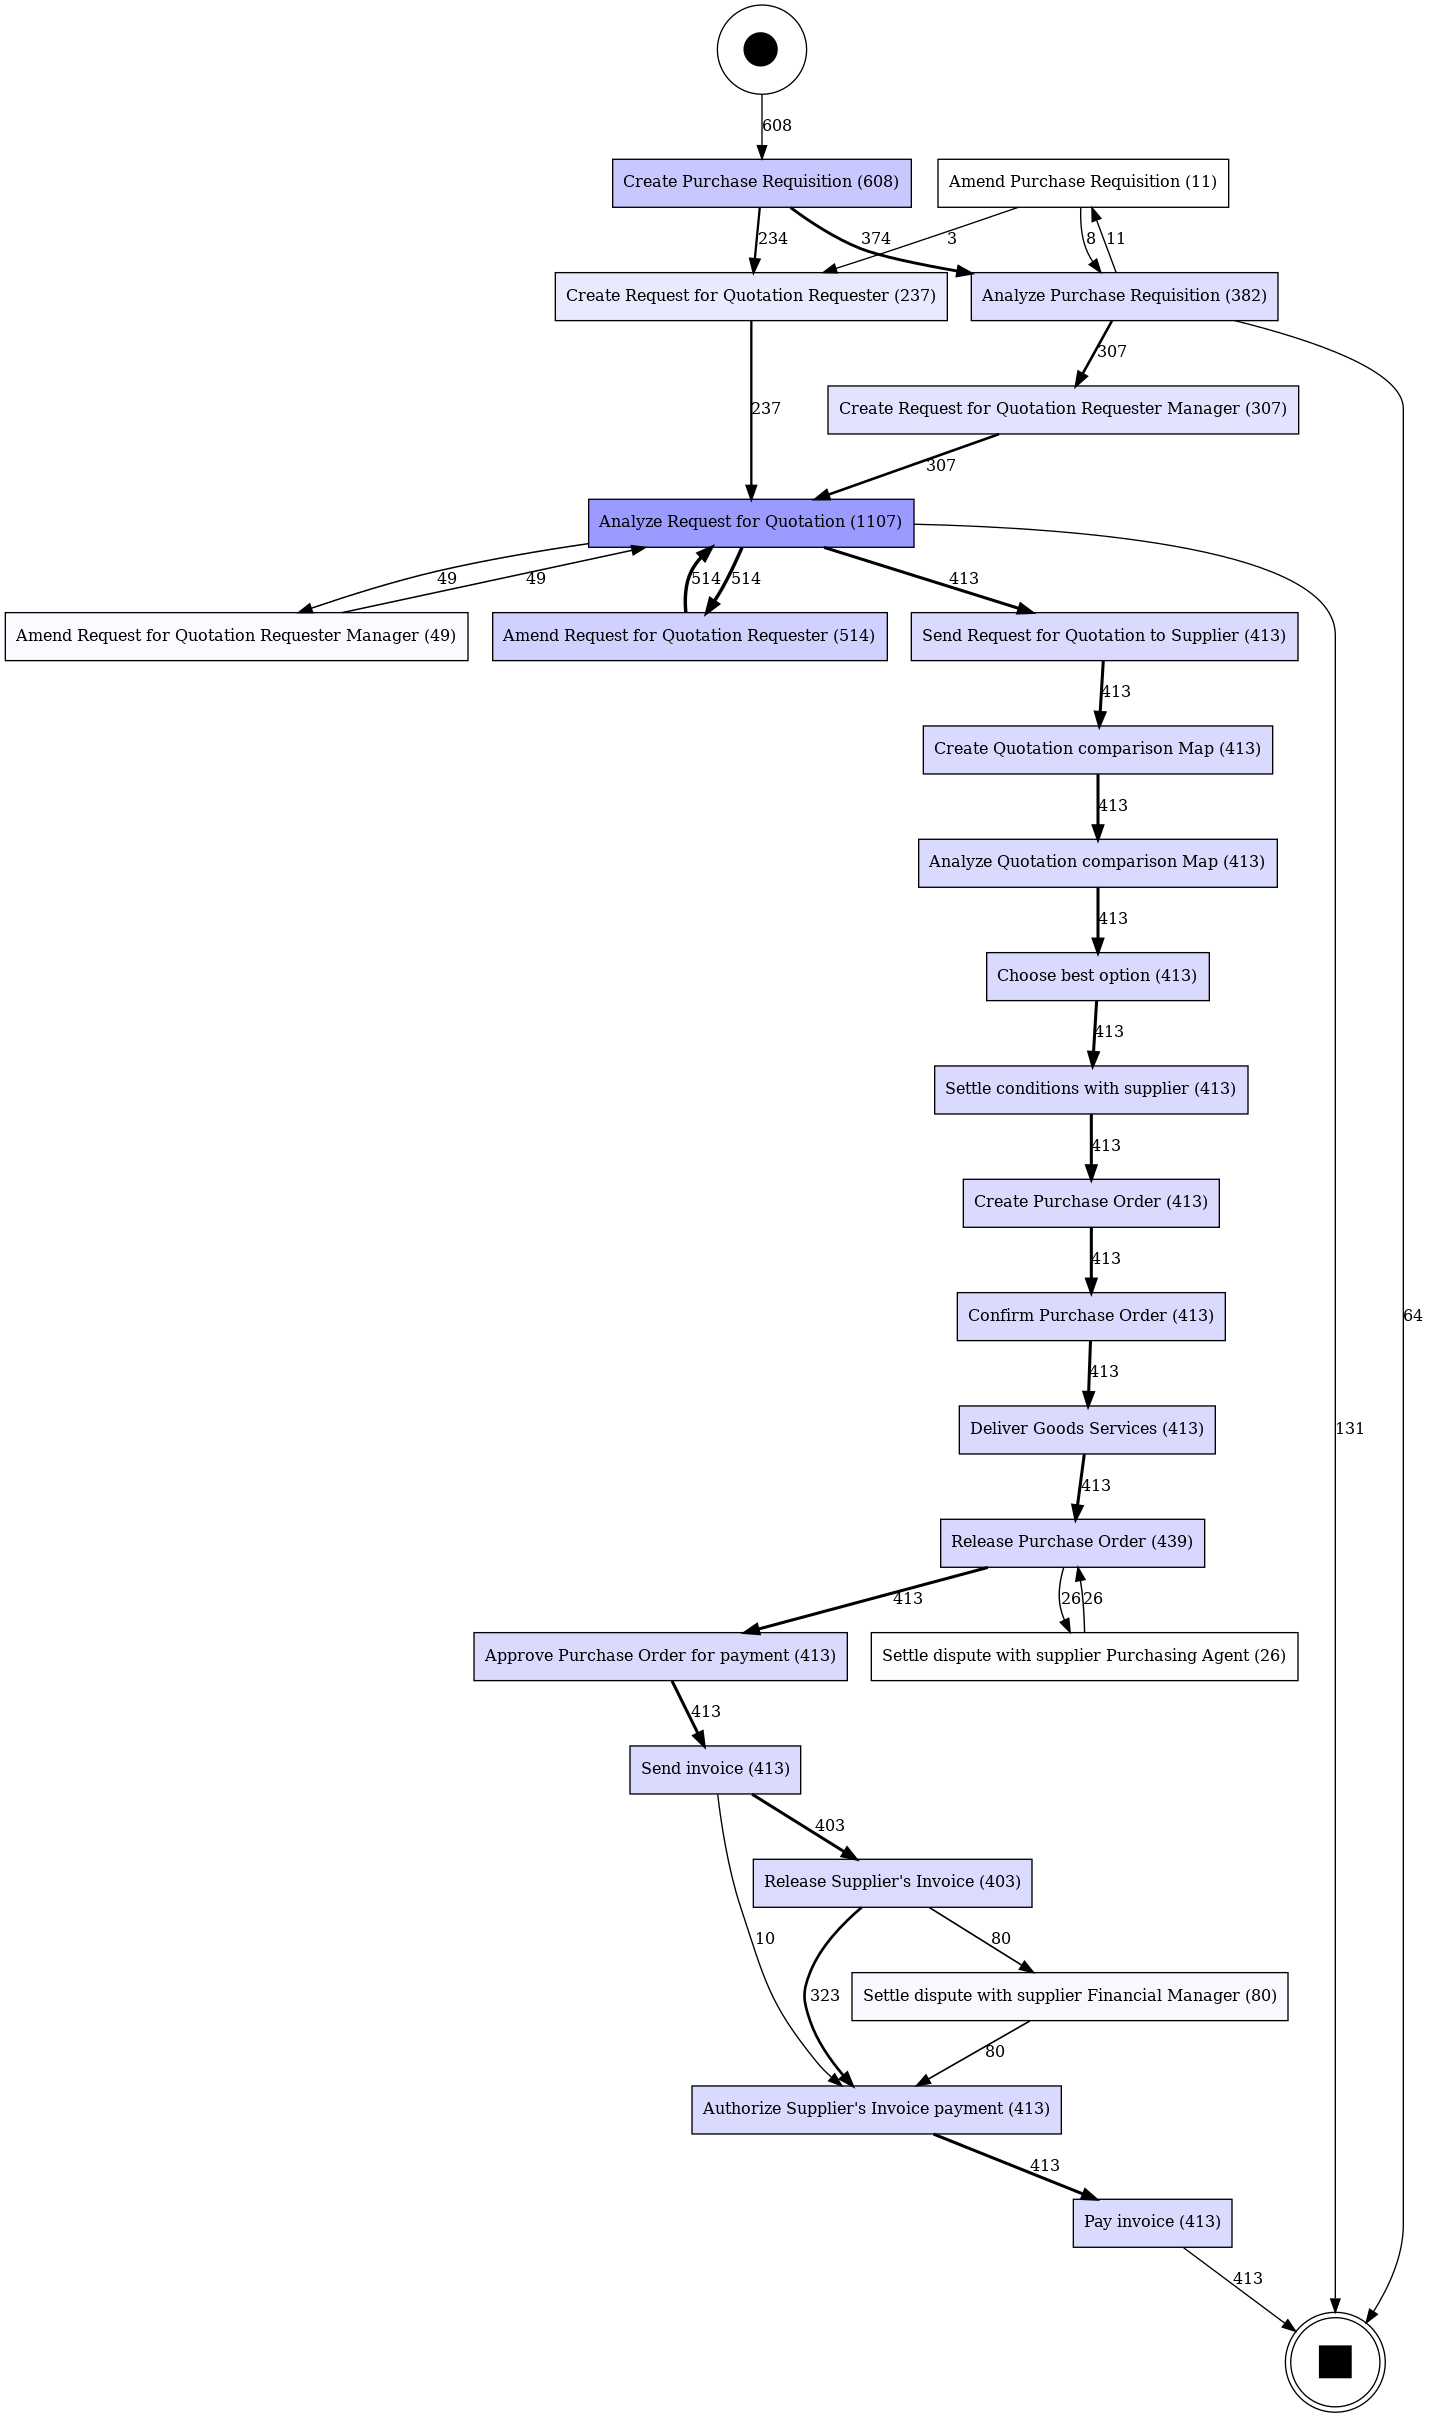
\includegraphics[width=.9\textwidth]{dfg.png}
\caption{Directly-Follows-Graph}
\label{fig:dfg}
\end{figure}

A DFG is not a process model in the sense of the example BPMN model in Figure~\ref{fig:bpmn}, as it is missing gateways and decisions. A range of algorithms have been developed over the years to discover BPMN models from event logs. PM4Py provides the Inductive Miner and the Heuristics Net Miner. 

The Inductive Miner\index{Inductive miner} works by repeatedly ''cutting'' the DFG for an event log to identify subsets of activities that represent exclusive choice, parallelism, sequence, or loops. For example, as Figure~\ref{fig:inductive} shows, when there are sets of activities that are not connected by each other, and have distinct pre- and post-sets of activities, then this may indicate an exclusive choice between these sets. Similarly, a sequence of activities is characterized by the absence of ''backwards'' connections in the DFG, and parallelism is indicated by a set of arrows that fully connects two sets of activities with a common post-set. 

\begin{figure}
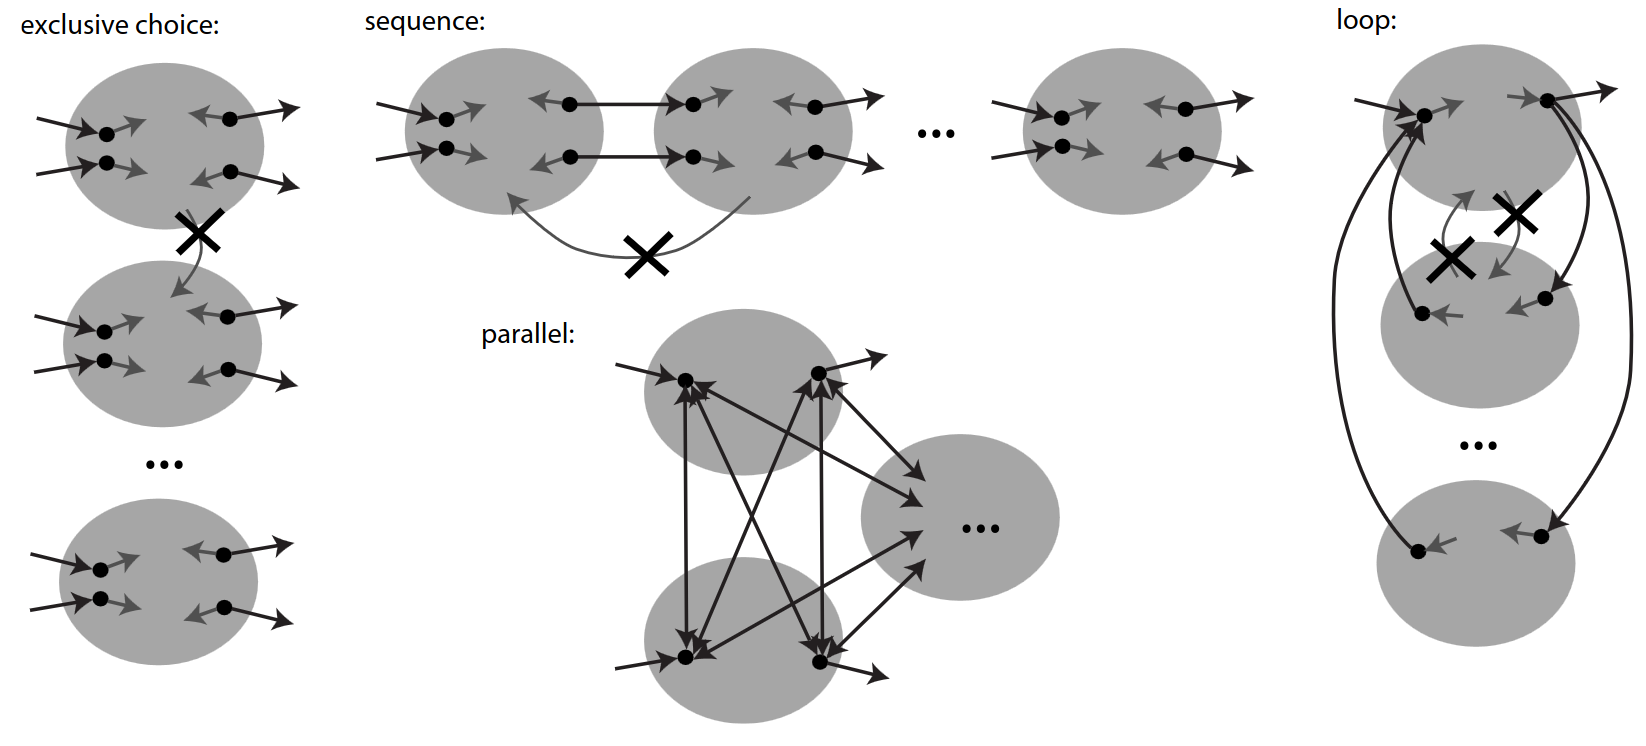
\includegraphics[width=\textwidth]{screen2.png}
\scriptsize 
Source: Leemans, S.J.J., Fahland, D., van der Aalst, W.M.P. (2013). Discovering Block-Structured Process Models from Event Logs - A Constructive Approach. In: Colom, JM., Desel, J. (eds) Application and Theory of Petri Nets and Concurrency. PETRI NETS 2013. Lecture Notes in Computer Science, vol 7927. Springer, Berlin, Heidelberg.
\caption{Principles of the Inductive Miner}
\label{fig:inductive}
\end{figure}

PM4Py provides the function \texttt{discover\_bpmn\_inductive} which produces a BPMN model that can be viewed and saved. An example is shown in Figure~\ref{fig:inductive_example}.

\begin{samepage}
\begin{pythoncode}
bpmn_model = pm4py.discover_bpmn_inductive(log, noise_threshold=0.5)

pm4py.view_bpmn(bpmn_model, rankdir='LR')

pm4py.save_vis_bpmn(bpmn_model, file_path='bpmn.png', rankdir='TB')
\end{pythoncode}
\end{samepage}

\begin{figure}
\centering
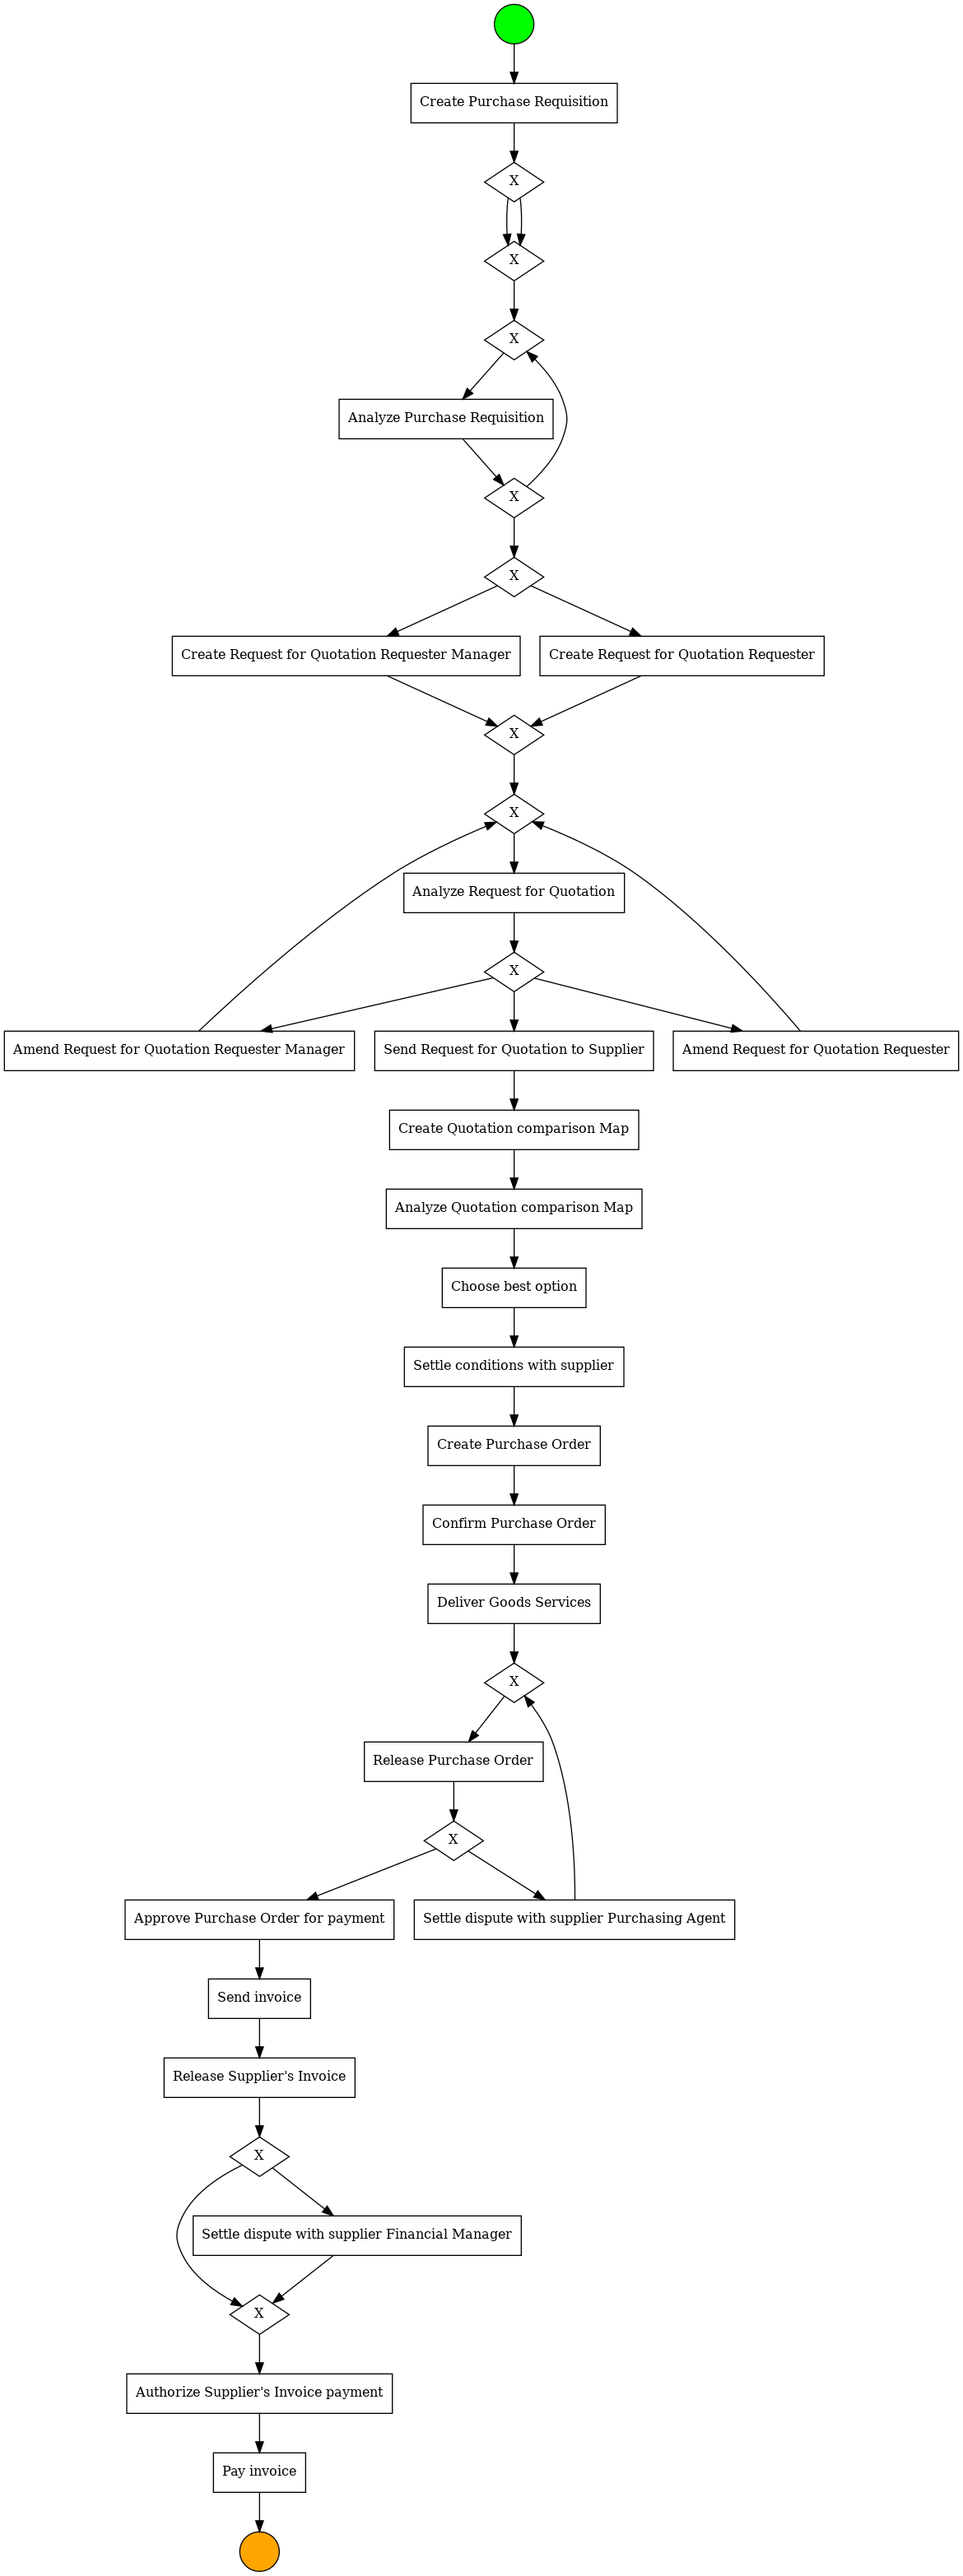
\includegraphics[height=7.25in]{bpmn.png}
\caption{Model discovered by the Inductive Miner}
\label{fig:inductive_example}
\end{figure}

In contrast, the Heuristics Net Miner \index{Heuristic net miner} focuses on frequencies in the DFG to identify sequences, parallelism, and loops. For example, a sequence between activities ''a'' and ''b'' by values larger than a threshold for the following proportion where the relation $a > b$ indicates the number of times $b$ follows $a$ in the DFG. Similar expressions exist to identify parallelism and loops. The thresholds are configurable; lower thresholds lead to the inclusion of more detail in the final model.

\begin{align*}
a \Rightarrow b = \left( \frac{
| a > b| - |b > a|}{
| a > b| + |b > a| + 1}\right)
\end{align*}
 
The PM4Py function \texttt{discover\_petri\_net\_heuristics} provides the Heuristics Net Miner. It returns a Petri net (a type of process model) that can be converted to a BPMN model for viewing and saving. An example is shown in Figure~\ref{fig:heuristics_example}.

\begin{samepage}
\begin{pythoncode}
petri_net, initial_marking, final_marking = \
    pm4py.discover_petri_net_heuristics(log, 
        dependency_threshold=0.6,
        and_threshold=0.65,
        loop_two_threshold=0.4)
        
pm4py.view_petri_net(petri_net)
        
bpmn_model2 = pm4py.convert_to_bpmn(petri_net, 
    initial_marking, final_marking)
    
pm4py.view_bpmn(bpmn_model2)
pm4py.save_vis_bpmn(bpmn_model2, 'bpmn2.png', rankdir='TB')
\end{pythoncode}
\end{samepage}

\begin{figure}
\centering
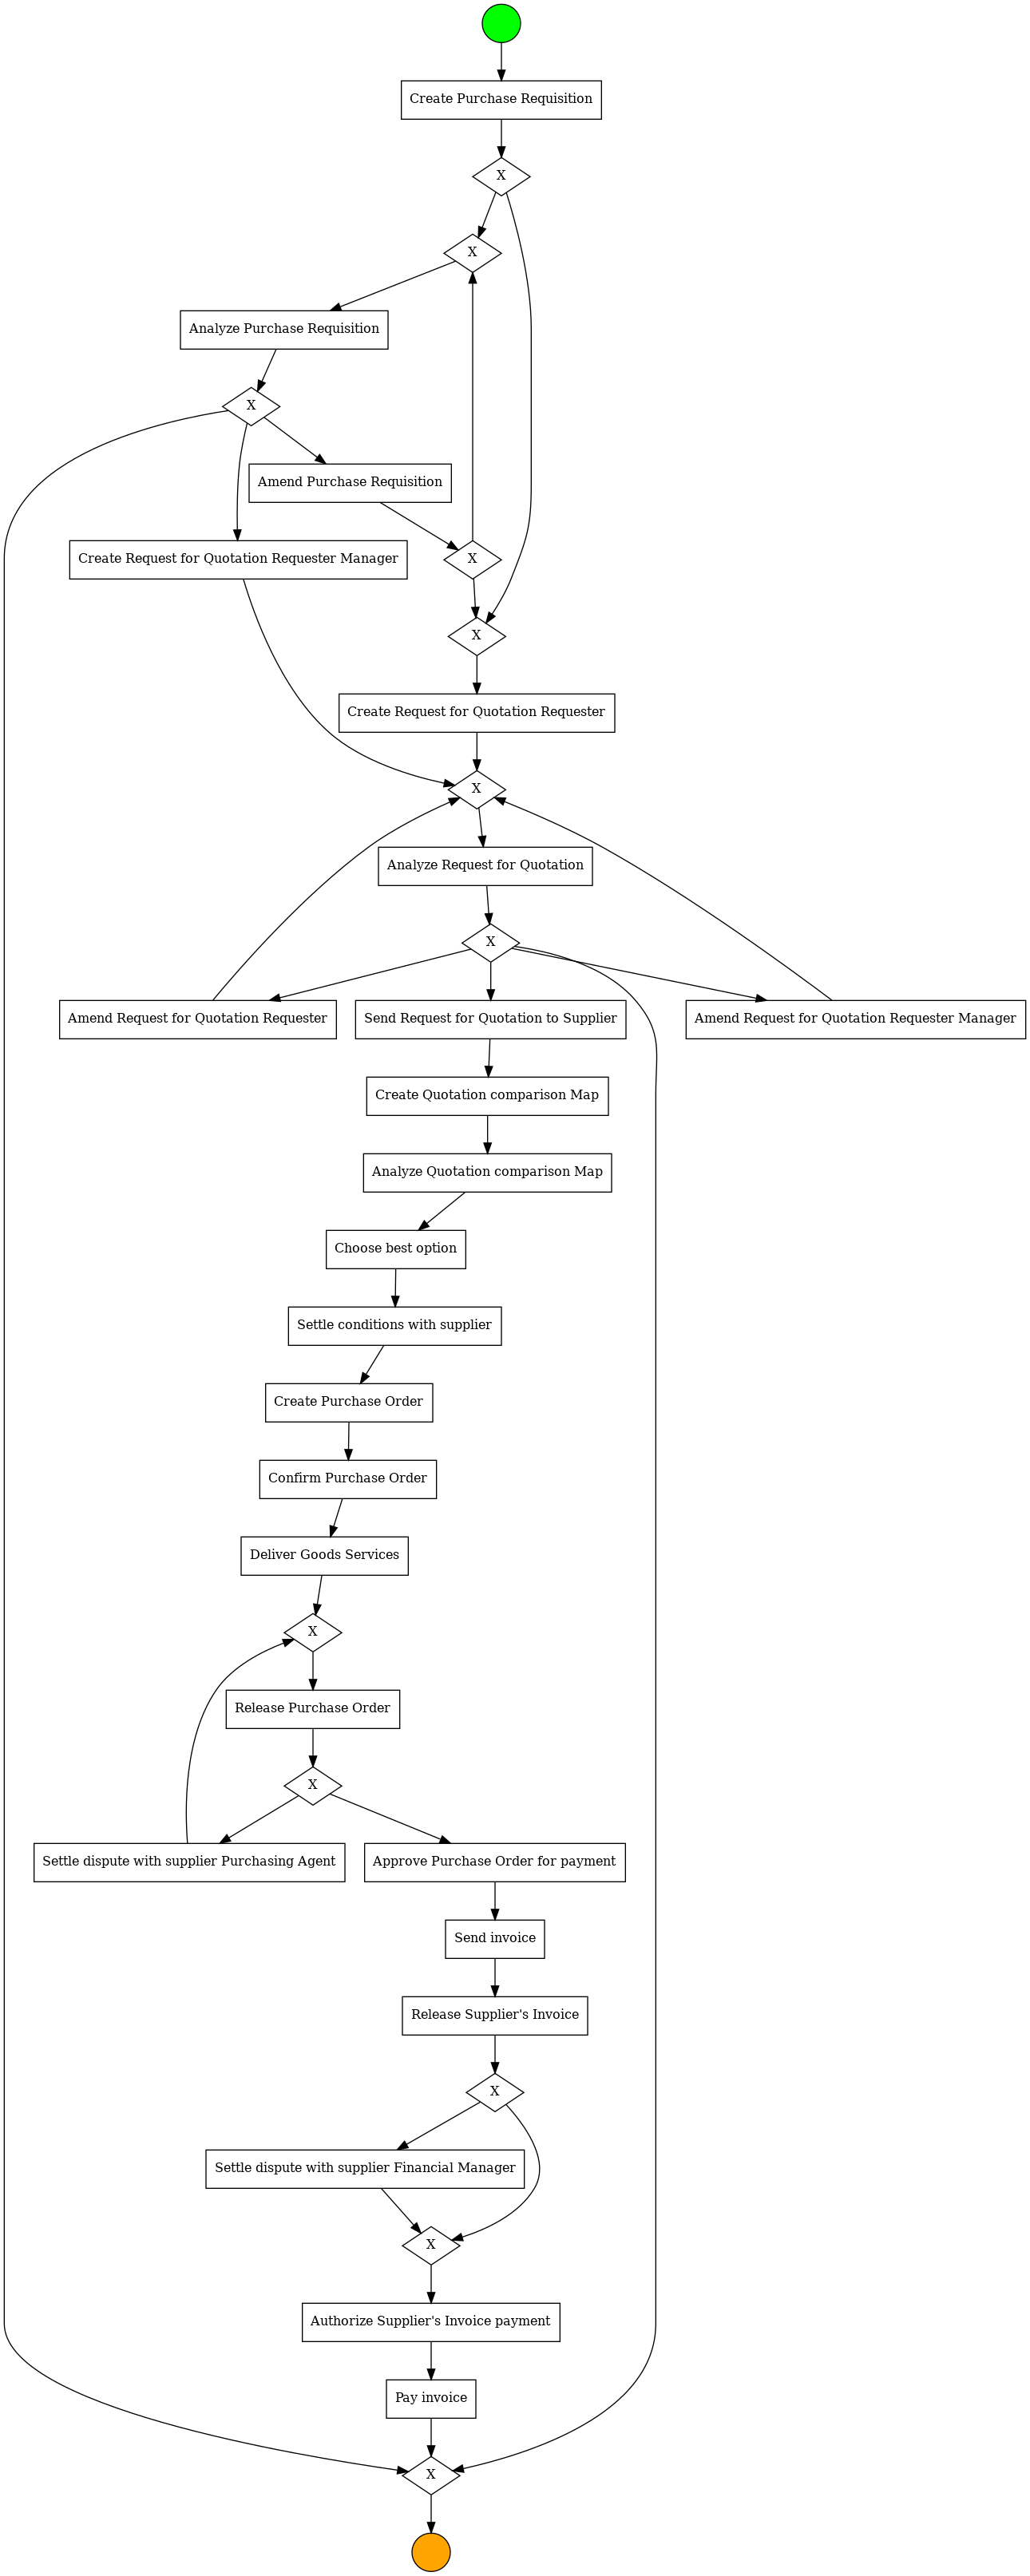
\includegraphics[height=7.25in]{bpmn2.png}
\caption{Model discovered by the Heuristics Net Miner}
\label{fig:heuristics_example}
\end{figure}

Once a model is automatically discovered from a log, the analyst must assess its quality. There are four aspects of model quality with respect to an event log:

\begin{itemize}
   \item \textbf{Fitness}: Can the model generate all traces in log?\index{Fitness}
   \item \textbf{Precision}: Does the model only generate traces in log?\index{Precision!in process discovery}
   \item \textbf{Generalization}: Can the model generalize to ''sensible'' traces not seen in log?
   \item \textbf{Complexity}: Is the model too complex to understand?
\end{itemize}

Quality assessment often focuses mainly on the calculation of fitness and precision, and two different techniques have been developed for this.

In \emph{token-based replay}\index{Token-based replay fitness}, each trace of an event log is replayed on the discovered process model using what is known as \emph{token semantics}. This discovers missing and surplus tokens, which represent model activities that cannot be executed, or model activities that are executed too often. Both cases indicate a mismatch between the model and the trace. The statistics of interest are the percentage of traces that fit the model perfectly, and the average fitness of all traces in the log.

\emph{Alignment-based fitness}\index{Alignment-based fitness} uses sequence alignment methods to align the model and each trace in an event log. It counts the the number of ''synchronous moves'' where an activity is both in a trace and the model, the number of ''move on log'' where an activity is in a trace but not in the model, and the number of ''move on model'' where an activity is in the model but not in the trace. The statistics of interest are also the percentage of traces that fit the model perfectly, and the average fitness of all traces.

Note that the results of the two types of analysis are not necessarily the same for all models and for all event logs.

PM4Py provides functions to compute fitness and precision using both methods. For this, PM4Py uses the Petri net type of process model. As we noted above, this can be transformed into a BPMN model for visualization. 

\begin{samepage}
\begin{pythoncode}
petri_net, initial_marking, final_marking = \
    pm4py.discover_petri_net_inductive(log, noise_threshold=0.5)

fitness_alignments = pm4py.fitness_alignments(log,
    petri_net, initial_marking, final_marking)
print(fitness_alignments)

fitness_tbr = pm4py.fitness_token_based_replay(log, 
    petri_net, initial_marking, final_marking)
print(fitness_tbr)

precision_alignments = pm4py.precision_alignments(log,
    petri_net, initial_marking, final_marking)
print(precision_alignments)

precision_tbr = pm4py.precision_token_based_replay(log, 
    petri_net, initial_marking, final_marking)
print(precision_tbr)
\end{pythoncode}
\end{samepage}

\subsection*{Log Filtering}

Filtering an event log prior to analysis is useful for three reasons. First, it allows the analyst to focus on a subset of the log information. For example, an analyst may wish to examine all traces of the order-to-cash process for domestic customers, or for business customers. Or an analyst may wish to examine only those cases that show some compliance problem. 

Second, filtering allows the analyst to split the event log in order to identify differences or similarities. For example, filtering the log of the order-to-cash process for domestic customers allows the analyst to identify differences in how domestic and overseas customer orders are processed. 

Third, filtering simplifies automatically discovered models. Many automatic discovery algorithms produce very complex models when the actual processes are complex or when there is a large amount of variation or noise in the event log. Noise does not necessarily mean invalid data, but data that appears infrequently or could be considered very atypical. Such noise, when included in the event log for process discovery, can ''clutter up'' the resulting model, making it difficult or impossible to understand.

PM4Py provides a number of different filters, with a few examples shown in Table~\ref{tab:pm4py_filters}. Information on other filters can be found on the PM4Py website.

\begin{table}
\small
\renewcommand{\arraystretch}{1.1}
\begin{tabularx}{\textwidth}{l|X} \hline 
\texttt{filter\_activities\_rework} & Keep cases where the specified activity occurs at least $n$ times \\
\texttt{filter\_case\_size} & Keep cases having a length between $n$ and $m$ events \\
\texttt{filter\_case\_performance} & Keep cases having a duration between $n$ and $m$ seconds \\
\texttt{filter\_directly\_follows\_relation} & Keep cases where $A$ is followed immediately by $B$ \\
\texttt{filter\_end\_activities} & Keep cases that end with the specified activity \\
\texttt{filter\_event\_attribute\_values} & Keep cases or events in cases that satisfy the specified condition \\ 
\texttt{filter\_eventually\_follows\_relation} & Keep cases where $A$ is eventually followed by $B$ \\
\texttt{filter\_start\_activities} & Keep cases that start with the specified activity \\
\texttt{filter\_time\_range} & Keep events occurring between two timestamps \\
\texttt{filter\_trace\_attribute\_values} & Keep cases that satisfy the specified condition \\ \hline
\end{tabularx}
\caption{Example event log filter functions in PM4Py}
\label{tab:pm4py_filters}
\end{table}

\begin{tcolorbox}[colback=code]
\subsubsection*{Hands-On Exercises -- Basic Log Information}

The following exercises are designed to be used with the event log in the running examples above. Tips are provided to guide you and to provide links to the documentation for important functions to use.

\begin{enumerate}
    \item What are the different types of activities in the log?
    \begin{itemize}
       \item Use the Pandas \href{https://pandas.pydata.org/docs/reference/api/pandas.unique.html}{\texttt{unique()}} function
    \end{itemize}
    \item How often does each activity occur in the log?
    \begin{itemize}
       \item Use the Pandas \href{https://pandas.pydata.org/pandas-docs/stable/reference/api/pandas.Series.value_counts.html}{\texttt{value\_counts()}} function
    \end{itemize}
    \item Filter the log for complete cases, that is, retain only those cases that end with activity ''Pay invoice''.
    \begin{itemize}
       \item Use \href{https://processintelligence.solutions/static/api/2.7.11/generated/pm4py.filtering.filter_end_activities.html}{\texttt{pm4py.filtering.filter\_end\_activities}}
    \end{itemize}
    \item Plot the case durations for the complete cases. What do you notice?
    \begin{itemize}
       \item Use \href{https://processintelligence.solutions/static/api/2.7.11/generated/pm4py.stats.get_all_case_durations.html}{\texttt{pm4py.stats.get\_all\_case\_durations}}
       \item Put case durations into a \texttt{pd.DataFrame}
       \item 1 day = 86400 seconds
       \item Use \href{https://plotly.com/python/histograms/}{\texttt{px.histogram}} or \href{https://processintelligence.solutions/static/api/2.7.11/generated/pm4py.vis.view_case_duration_graph.html}{\texttt{pm4py.vis.view\_case\_duration\_graph}}
    \end{itemize}
    \item What is the mean case duration?
    \begin{itemize}
       \item Use the Pandas \href{https://pandas.pydata.org/docs/reference/api/pandas.DataFrame.mean.html}{\texttt{mean()}} function on the result of the previous exercise
    \end{itemize}
\end{enumerate}
\end{tcolorbox}

\begin{tcolorbox}[colback=code]
\subsubsection*{Hands-On Exercises for PM4Py -- Automatic Process Discovery}

The following exercises are designed to be used with the event log in the running examples above. Tips are provided to guide you and to provide links to the documentation for important functions to use.

\begin{enumerate}
    \item Using the mean case duration identified in the previous exercise, split the log on the mean case duration; that is, one sub-log should contain traces that are shorter than the mean, the other sub-log should contain cases that take longer than the mean.
    \begin{itemize}
       \item Use \href{https://processintelligence.solutions/static/api/2.7.11/generated/pm4py.filtering.filter_case_performance.html}{\texttt{pm4py.filtering.filter\_case\_performance}}
    \end{itemize}
    \item Discover BPMN models for each partial log and compare them. How do they differ?
    \item Discover a BPMN model from the total log. How does it differ from the models discovered for the partial logs?
    \item Calculate and compare the fitness and precision values of the models discovered from the partial log and the total log.
\end{enumerate}
\end{tcolorbox}

\begin{tcolorbox}[colback=code]
\subsubsection*{Hands-On Exercises for PM4Py -- Performance Analysis}

The following exercises are designed to be used with the event log in the running examples above. Tips are provided to guide you and to provide links to the documentation for important functions to use.

\begin{enumerate}
   \item What is the activity with the longest mean time? Activities taking a long time may be a bottleneck in the process flow.
   \begin{itemize}
       \item Create a new column as the difference between the 'Complete Timestamp' and 'start\_timestamp' columns.
       \item Use the Pandas \href{https://pandas.pydata.org/docs/reference/api/pandas.DataFrame.groupby.html}{\texttt{groupby()}} and \href{https://pandas.pydata.org/docs/reference/api/pandas.DataFrame.mean.html}{\texttt{mean()}} functions to group the data frame by activity.
   \end{itemize}
   \item What is the mean number of activities for each case? Long cases with many activities may indicate problems or overly complex processes.
   \begin{itemize}
       \item Calculate the number of activities for each case using the Pandas \href{https://pandas.pydata.org/docs/reference/api/pandas.DataFrame.groupby.html}{\texttt{groupby()}} and \href{https://pandas.pydata.org/docs/reference/api/pandas.DataFrame.count.html}{\texttt{count()}} functions on the dataframe
   \end{itemize}
   \item Which activities are carried out more than once for some case? Repeated activities may indicate re-work or fixing of mistakes.
   \begin{itemize}
       \item Calculate the number of instances for each case for each activity using the Pandas \href{https://pandas.pydata.org/docs/reference/api/pandas.DataFrame.groupby.html}{\texttt{groupby()}} and \href{https://pandas.pydata.org/docs/reference/api/pandas.DataFrame.count.html}{\texttt{count()}} functions on the dataframe
   \end{itemize}
\end{enumerate}
\end{tcolorbox}

\begin{tcolorbox}[colback=code]
\subsubsection*{Hands-On Exercises for PM4Py -- Conformance Analysis}

The following exercises are designed to be used with the event log in the running examples above. Tips are provided to guide you and to provide links to the documentation for important functions to use.

\begin{enumerate}
   \item Are there cases that contain activity ''Pay invoice'' but do not contain activity ''Send invoice''? Non-compliant cases may represent a problem with controls and compliance.
   \begin{itemize}
      \item Use \href{https://processintelligence.solutions/static/api/2.7.11/generated/pm4py.filtering.filter_eventually_follows_relation.html}{\texttt{filter\_eventually\_follows\_relationship}}
   \end{itemize}
\end{enumerate}
\end{tcolorbox}

\section{Performance Mining}

Performance mining\index{Performance mining} is that aspect of process analytics that analyzes the temporal performance of a process. Information of interest are the durations of the activities (\emph{service time}\index{Service time}), the \emph{waiting times}\index{Waiting time} between activities, and the overall case durations. For each of those, different summary statistics are useful, such as the mean, median, standard deviation, maximum and minimum. 

The easiest and most interpretable way to do this in PM4Py is to annotate the DFG with this information. For example, the following Python code block calculates the median waiting times between activities and shows them in the DFG. The annotated DFG is shown in Figure~\ref{fig:performance_dfg}. Because the example event log did not contain start and end times for each activity, it is not possible to show the service times on the DFG, that is, the duration of the activities.

\begin{samepage}
\begin{pythoncode}
perf_dfg, start_activities, end_activities = \
    pm4py.discover_performance_dfg(log)
    
pm4py.view_performance_dfg(perf_dfg, 
    start_activities, end_activities, 
    aggregation_measure='median')

pm4py.save_vis_performance_dfg(perf_dfg, 
    start_activities, end_activities, 
    file_path='perfdfg.png', rankdir='TB')
\end{pythoncode}
\end{samepage}

This example shows a few problems with the process. For example, the median wait time between creating a request for quotation and analyzing it is 6 days. If the request needs to be amended, it then has to wait another 8 to 10 days to be analyzed again. These long wait times indicate performance problems in the process. This may stem from a lack of resources, or insufficient prioritization, or other process issues, that needs be investigated in detail by the process analyst. 

\begin{figure}
\centering

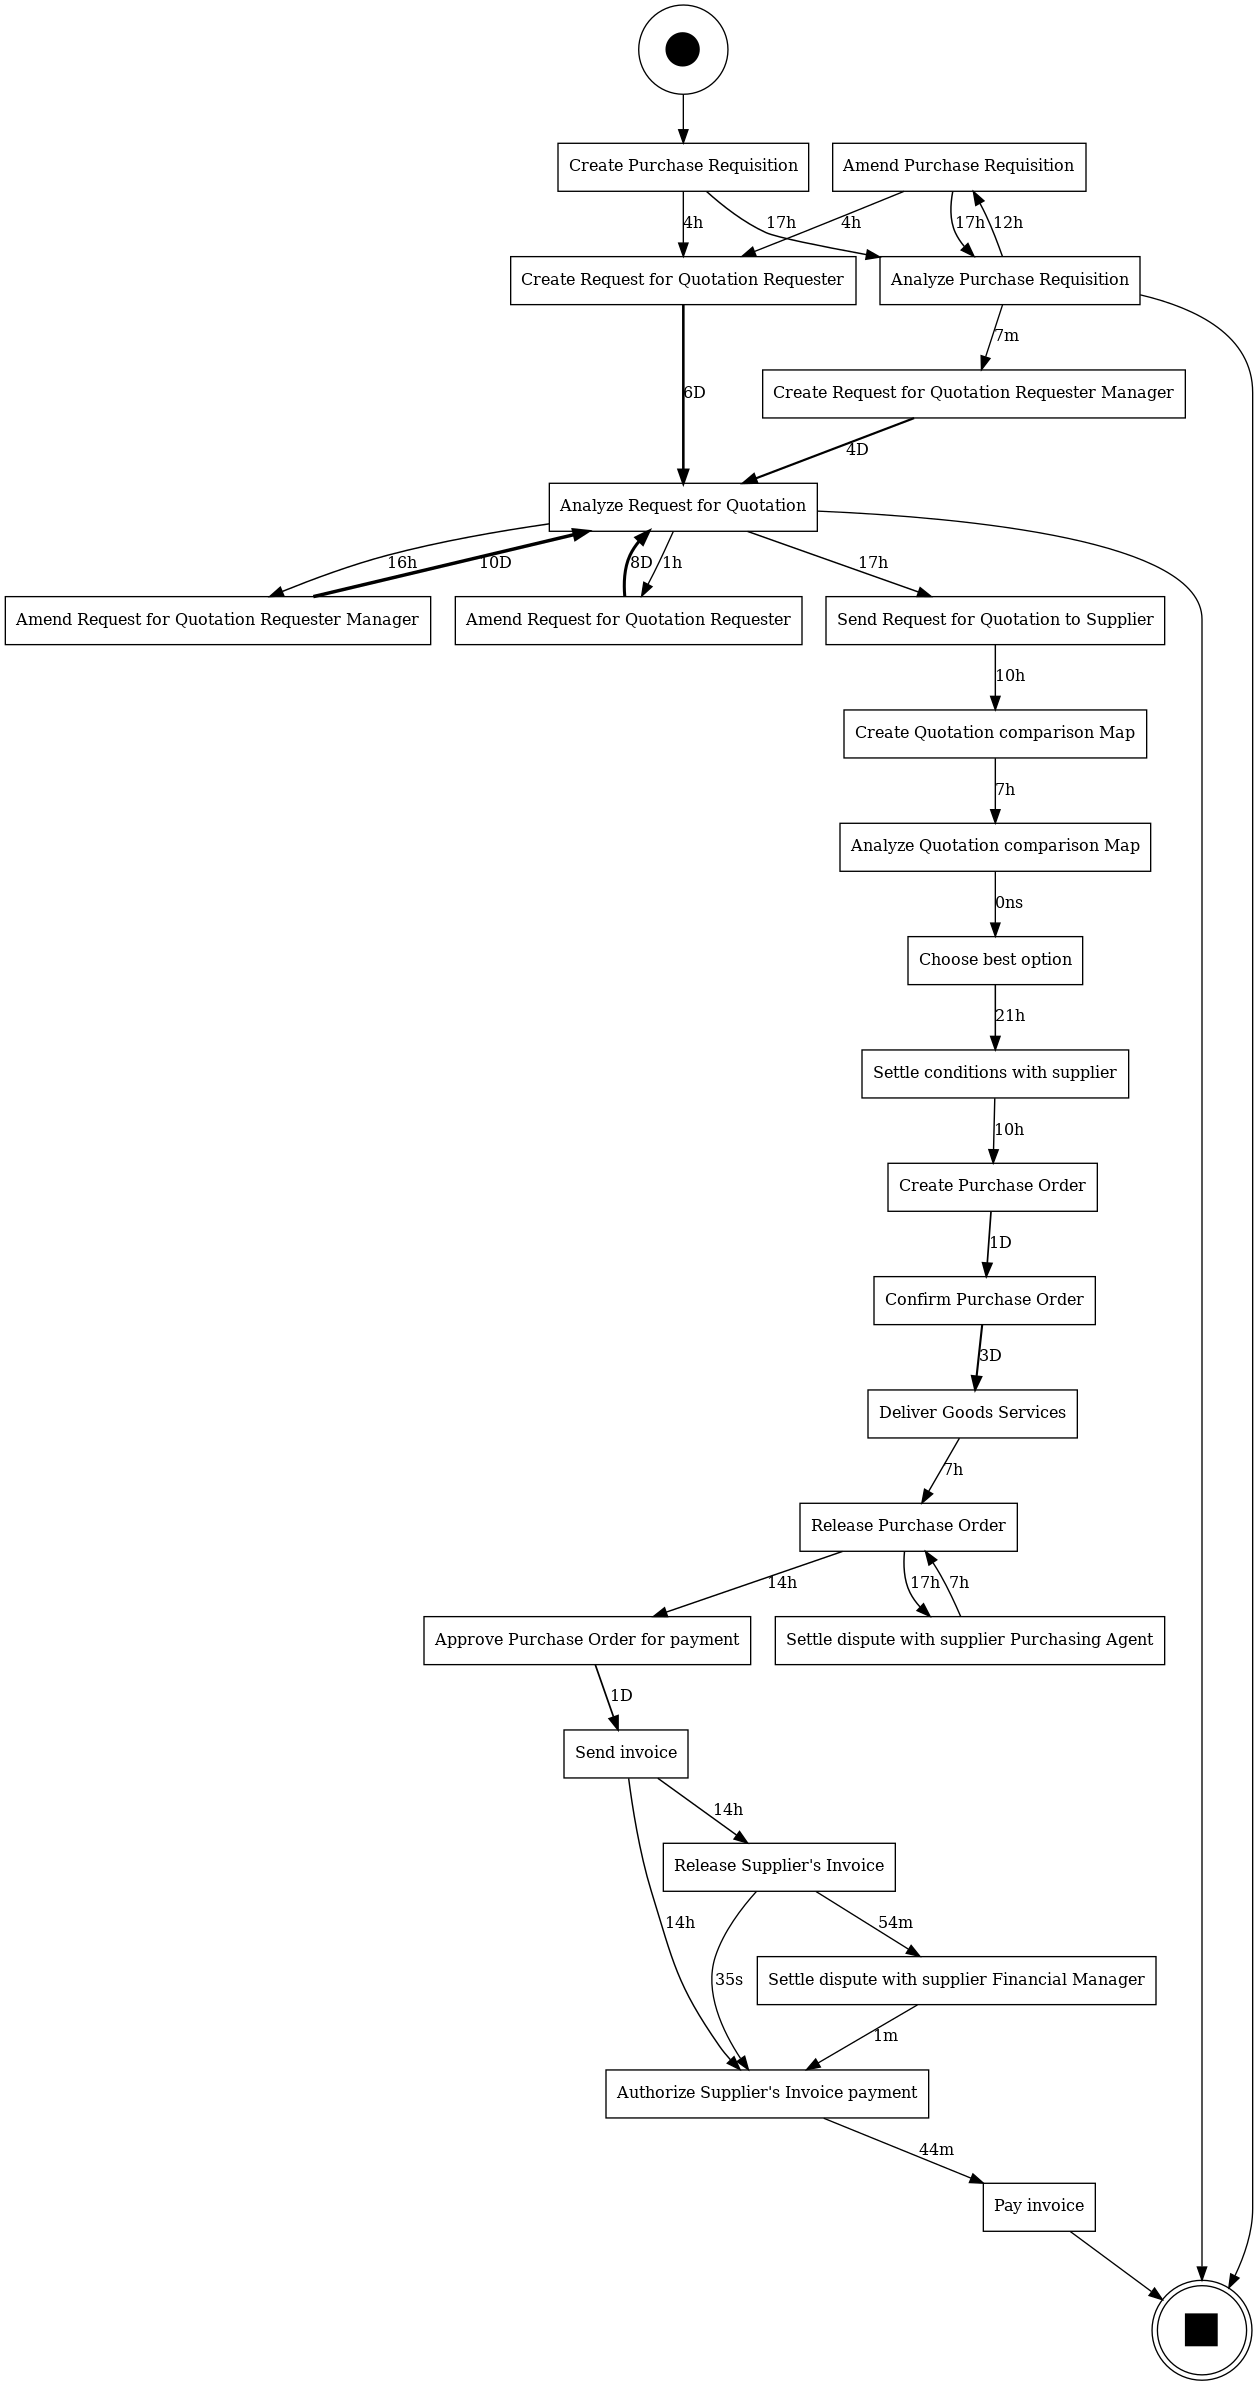
\includegraphics[height=7.25in]{perfdfg.png}
\caption{DFG annotated with median waiting times}
\label{fig:performance_dfg}
\end{figure}

Another useful tool in process performance analysis is the \emph{dotted chart}\index{Dotted chart}. An example dotted chart is shown in Figure~\ref{fig:dotted_chart}. The horizontal axis represents the time stamp of each activity or event, while the vertical axis represents the case ID -- each row in the diagram contains the events of one trace. The colors correspond to different types of activities. The following Python code produces the example in Figure~\ref{fig:dotted_chart}.

\begin{samepage}
\begin{pythoncode}
perf_dfg, start_activities, end_activities = \
    pm4py.discover_performance_dfg(log)
    
pm4py.view_performance_dfg(perf_dfg, 
    start_activities, end_activities, 
    aggregation_measure='median')
    
pm4py.save_vis_performance_dfg(perf_dfg, 
    start_activities, end_activities, 
    file_path='perfdfg.png', rankdir='TB')
\end{pythoncode}
\end{samepage}

\begin{figure}
\centering
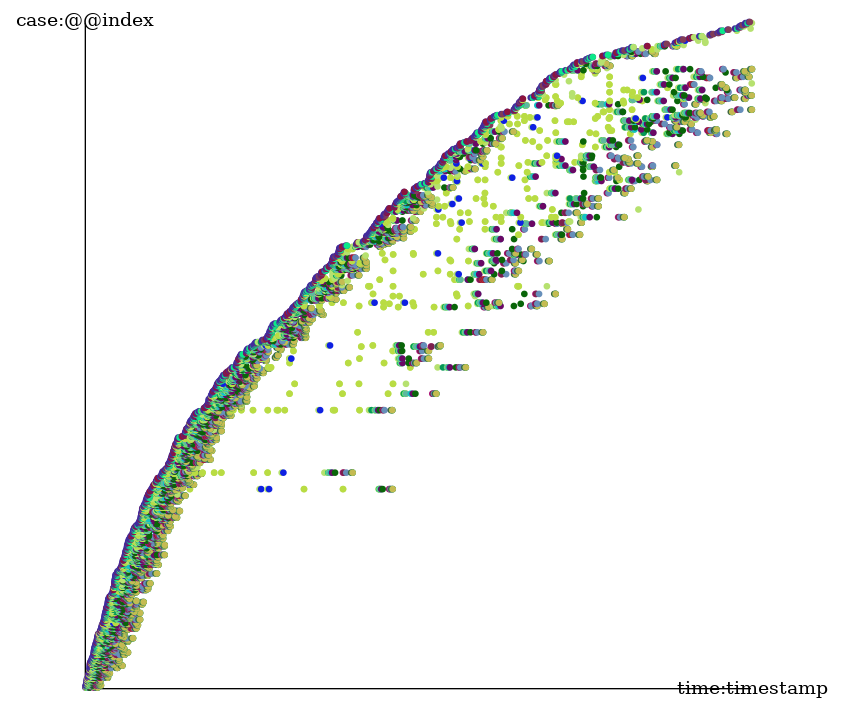
\includegraphics[width=.8\textwidth]{dottedchart.png}
\caption{Example of a Dotted Chart}
\label{fig:dotted_chart}
\end{figure}

A dotted chart can be used to show batching of activities, that is, activities in different cases that are not spread out in time but are executed at the same time. This may indicate that some cases have to wait for the next batch to be processed, leading to potential delays. A dotted chart can also show different variants, by visually highlighting different types of performance. In the example of Figure~\ref{fig:dotted_chart}, it is clear that many cases are finished quickly, while others take a long time. In particular, the cases that arrive early or very late in the log tend to be those that finish quickly. 

A dotted chart can also be useful to examine the case arrival rates. In the example in Figure~\ref{fig:dotted_chart} it is clear that early in time, cases arrive more frequently than later in time (the curve is steeper there). This may indicate a shift in the demand for a particular product or service. 

A performance spectrum graph\index{Performance spectrum graph}, like the one in Figure~\ref{fig:perf_spectrum} shows the wating times between two activities, the one at the top and the one at the bottom. The horizontal axis represents time. Lines that are slanted or run diagonally at an angle indicate a long waiting time. A performance spectrum can also show when lines are ''bunched together'' or ''sparsely distributed'', indicating variations in the rate at which one activity finishes or the next activity begins. The following Python code block produces the graph in Figure~\ref{fig:dotted_chart}.

\begin{samepage}
\begin{pythoncode}
pm4py.view_performance_spectrum(log,
    ['Send invoice', 'Pay invoice'])

pm4py.save_vis_performance_spectrum(log,
    ['Send invoice', 'Pay invoice'],
    'perfspectrum.png') 
\end{pythoncode}
\end{samepage}

\begin{figure}
\centering
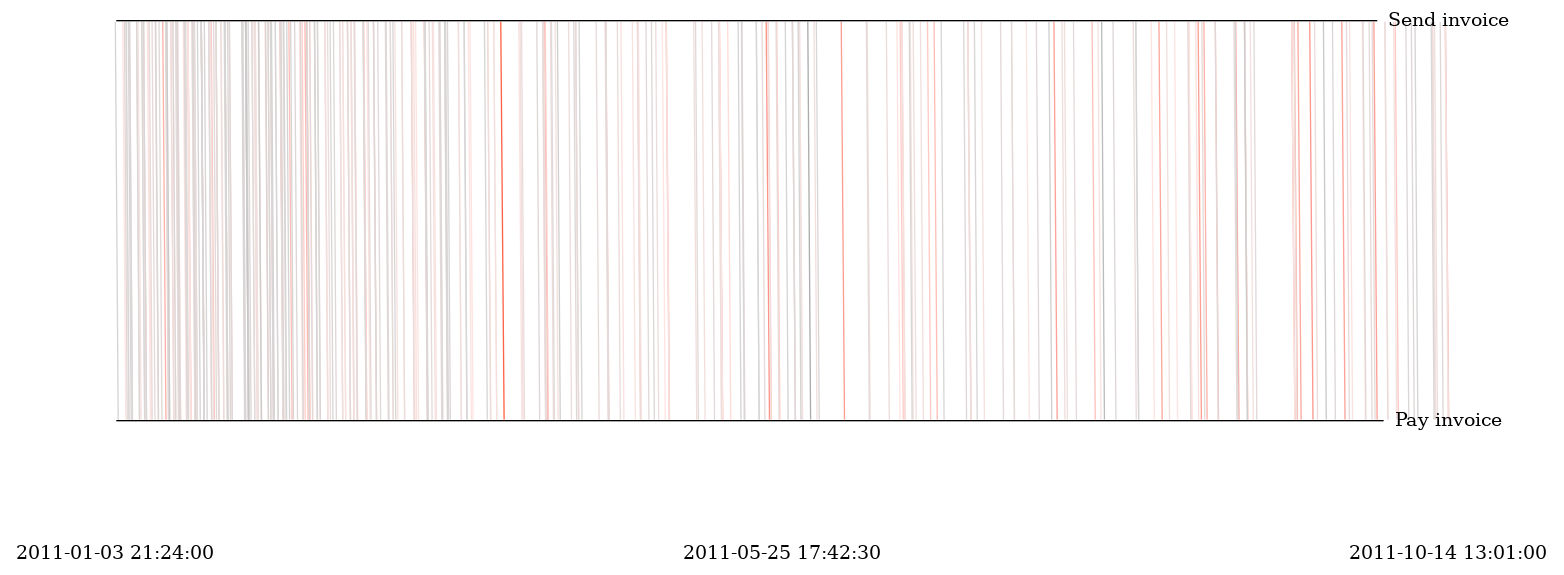
\includegraphics[width=.9\textwidth]{perfspectrum.png}
\caption{Example of a Performance Spectrum}
\label{fig:perf_spectrum}
\end{figure}

To indicate when a process that delivers a service is in high demand and requires high capacity, the distribution of events over time should be considered. This can be done by day-of-the-week, by month-of-the-year, or by week-of-the-year, as the following PM4Py functions show. An example of event distribution by week-of-the-year is shown in Figure~\ref{fig:event_distribution}.

\begin{samepage}
\begin{pythoncode}
pm4py.view_events_distribution_graph(log, 'days_week')
pm4py.view_events_distribution_graph(log, 'days_month')
pm4py.view_events_distribution_graph(log, 'months')
pm4py.view_events_distribution_graph(log, 'weeks')
\end{pythoncode}
\end{samepage}

The example in Figure~\ref{fig:event_distribution} shows that this process is very busy early in the year, in approximately the first quarter, but not at all in the last quarter of the year, except for some activity in the final week of the year. This uneven demand requires adequate capacity planning over of the organization and an organization may decide to identify ways to smooth out the demand. 

\begin{figure}
\centering
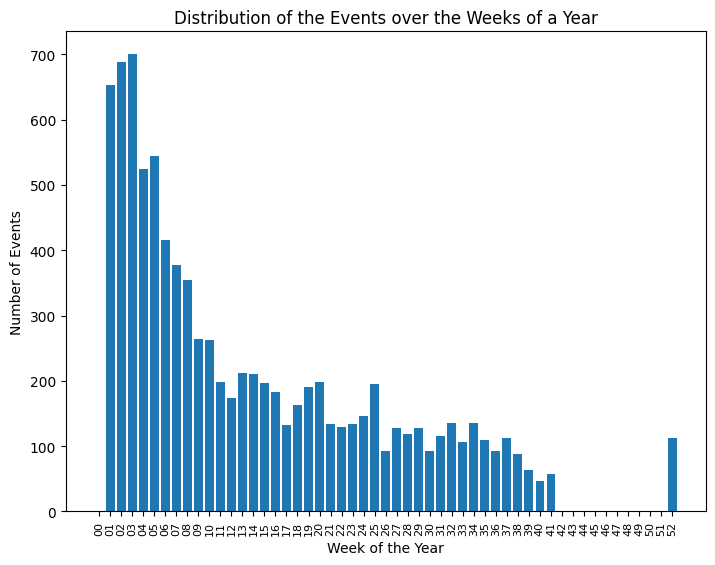
\includegraphics[width=.7\textwidth]{eventsdistribution.png}
\caption{Event distribution over time}
\label{fig:event_distribution}
\end{figure}

Plotting the events over time for the entire log as a probability density shows similar characteristics. Figure~\ref{fig:events_per_time} plots the frequency (technically, a probability kernel density) of event occurrence, produced by the following Python code.

\begin{samepage}
\begin{pythoncode}
pm4py.view_events_per_time_graph(log)
pm4py.save_vis_events_per_time_graph(log, 'eventspertime.png')
\end{pythoncode}
\end{samepage}

\begin{figure}
\centering
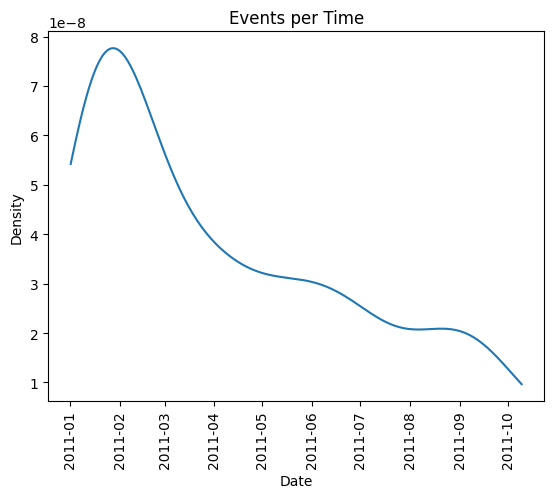
\includegraphics[width=.7\textwidth]{eventspertime.png}
\caption{Events per time graph}
\label{fig:events_per_time}
\end{figure}

\FloatBarrier
\section{Organizational Mining}

Organizational mining focuses on the resources and their roles in a process. It uses the data in an event log to identify how resources and roles work together to execute process instances. 

A simple way to focus on organizational roles or resources is to construct a DFG, but using the resource or role information for the nodes of the graph, instead of the activity names. The DFG then expresses how often one resource or role follows another in the execution of the cases; in other words, how often one resource or role passes work to another (or to itself). The following Python code block produces the \emph{handover-of-work network}\index{Handover-of-work network} shown in Figure~\ref{fig:handover}. Notice how the same PM4Py function for the DFG discovery is used, but a different data frame column is specified for the ''activity\_key'' parameter.

\begin{samepage}
\begin{pythoncode}
dfg, start, end = pm4py.discover_dfg(log, activity_key='Role')

pm4py.view_dfg(dfg, start, end, rankdir='LR')

pm4py.save_vis_dfg(dfg=dfg,
    start_activities=start, 
    end_activities=end, 
    file_path='handover.png', rankdir='TB')
\end{pythoncode}
\end{samepage}

\begin{figure}
\centering
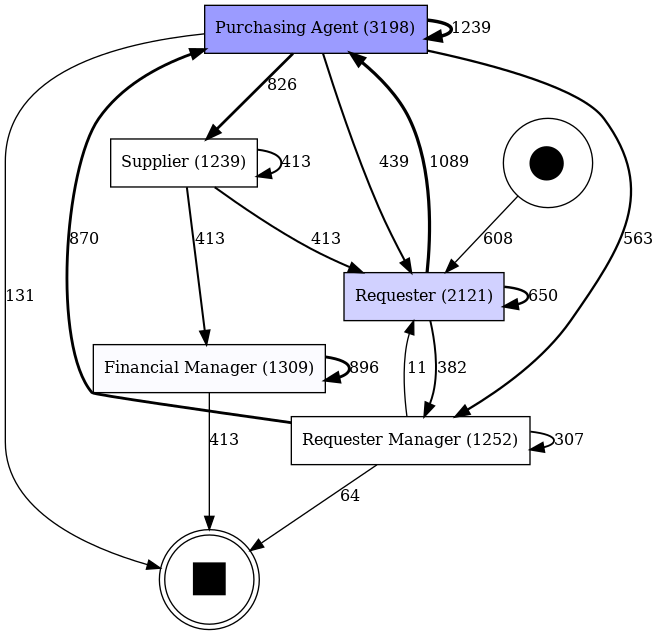
\includegraphics[width=.66\textwidth]{handover.png}
\caption{Example handover-of-work network}
\label{fig:handover}
\end{figure}

A similar analysis can be performed using the PM4Py function \\ \texttt{discover\_working\_together\_network()}, as shown in the following Python code and in Figure~\ref{fig:workingtogether}. Note that this graph is normally interactive.

\begin{samepage}
\begin{pythoncode}
sna_graph = pm4py.discover_working_together_network(log,
   resource_key='Role')
pm4py.view_sna(sna_graph, variant_str='pyvis')   
pm4py.view_sna(sna_graph, variant_str='networkx')   
\end{pythoncode}
\end{samepage}

\begin{figure}
\centering
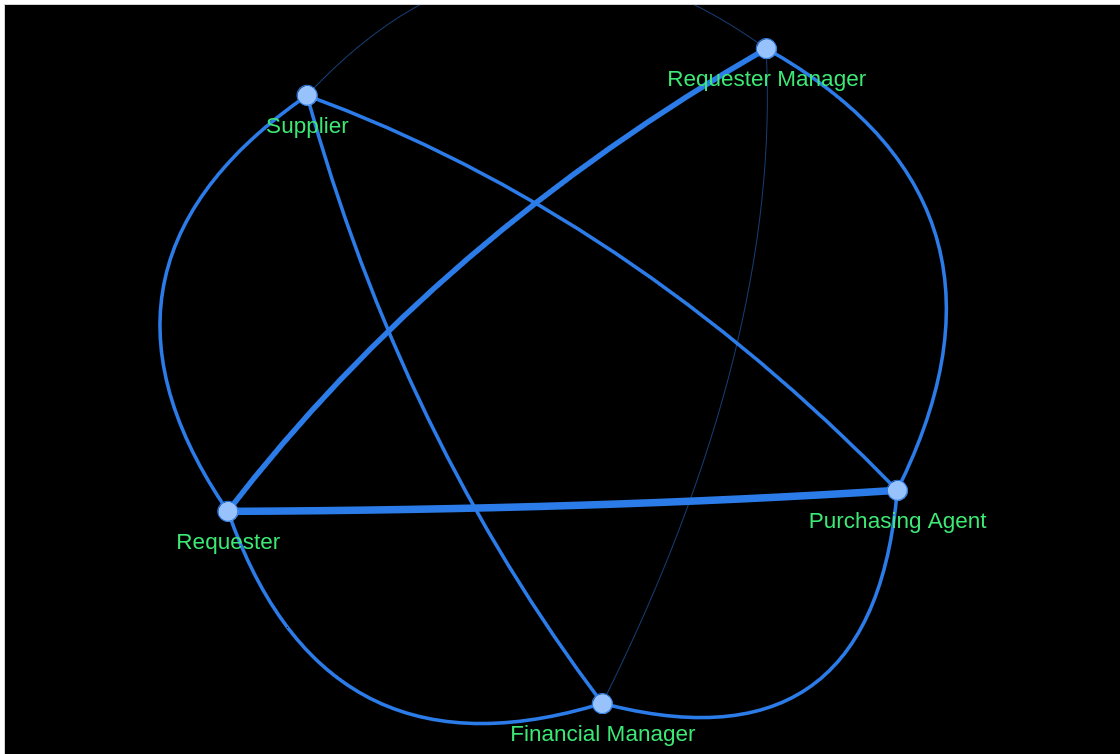
\includegraphics[width=.66\textwidth]{screen4.png}
\caption{Example working-together network}
\label{fig:workingtogether}
\end{figure}

Yet another analysis focuses on identifying resources that perform the same sets of activities. This is useful for identifying implicit roles or resources with similar skills.

\begin{samepage}
\begin{pythoncode}
roles = pm4py.discover_organizational_roles(log)
print(roles)
\end{pythoncode}
\end{samepage}

Another way to achieve this goal is with the following Python code, which produces the activity-based resource similarity graph in Figure~\ref{fig:resource_similarity}. The graph shows four clusters of resources that are similar to each other within their cluster, i.e. they perform similar sets of activities in this process. 

\begin{samepage}
\begin{pythoncode}
sna_graph = pm4py.discover_activity_based_resource_similarity(log)

pm4py.view_sna(sna_graph, variant_str='networkx')
pm4py.view_sna(sna_graph, variant_str='pyvis')

pm4py.save_vis_sna(sna_graph, 'ressimilarity.png',
    variant_str='networkx')
\end{pythoncode}
\end{samepage}

\begin{figure}
\centering
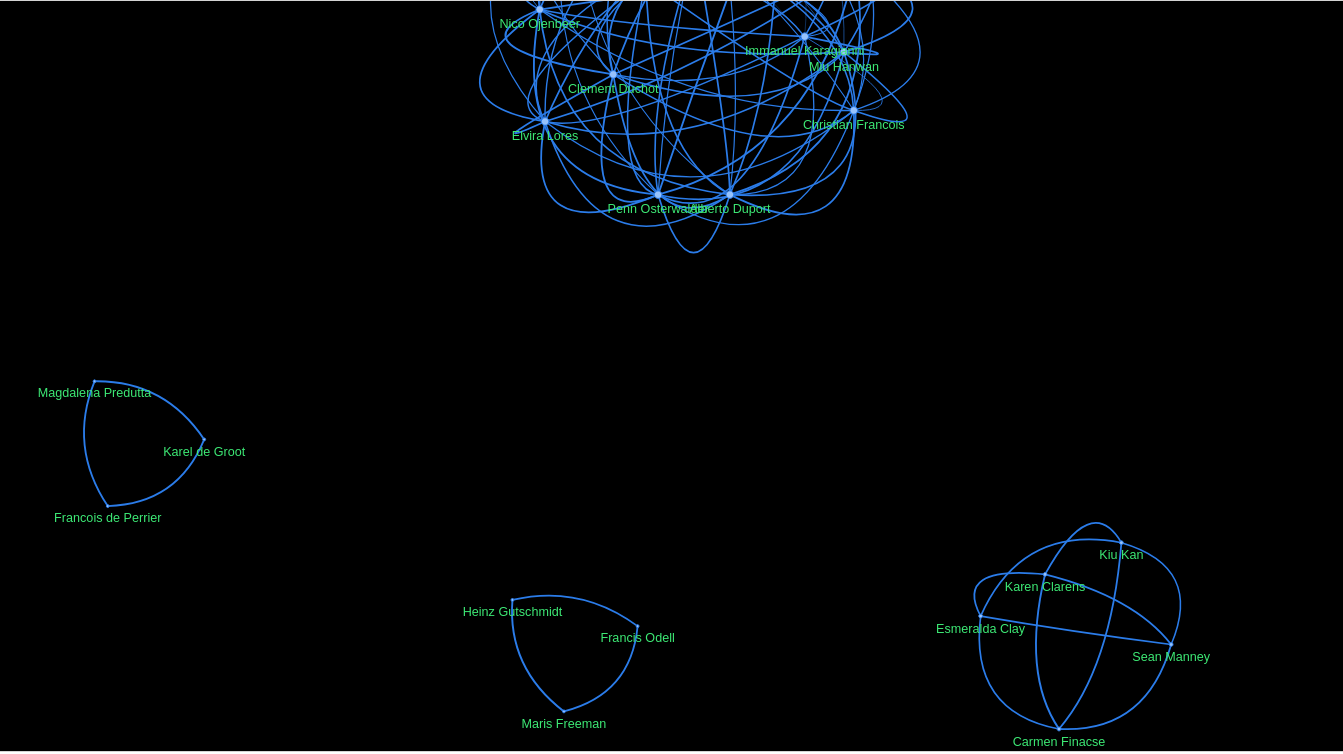
\includegraphics[width=.66\textwidth]{screen3.png}
\caption{Activity-based resource similarity graph}
\label{fig:resource_similarity}
\end{figure}

\section{Review Questions}

The following review questions help you evaluate your understanding of this material.

\begin{enumerate}[nosep]
    \item What is business process analytics and why is it important in improving operational efficiencies?
    \item Define a business process. What are the typical elements that constitute a business process?
    \item What roles do resources play in a business process? Provide examples.
    \item What is the Business Process Modeling Notation (BPMN)? Why is it widely used?
    \item Explain the symbols used in BPMN to represent events, activities, gateways, and dependencies.
    \item Describe the function of an exclusive gateway in a BPMN diagram. Provide an example from the given material.
    \item Explain what a parallel gateway is and provide an example of how it is used in business process modeling.
    \item What is an inclusive gateway? Give an example of its application in a business process.
    \item Given a simple process scenario, draw a BPMN diagram using appropriate symbols for events, activities, and gateways.
    \item Define a ''case'' in the context of a business process. Provide an example.
    \item What is a ''trace''? How does it relate to a case?
    \item Explain the term ''event'' in process mining. What might an event signify in a business process event log?
    \item Describe the typical lifecycle of an activity in a business process. Refer to the XES standard lifecycle model.
    \item What are some possible states and transitions an activity might go through during its lifecycle?
    \item Differentiate between ''event attributes'' and ''case attributes.'' Provide examples of each.
    \item Why is it important to associate events with resources and timestamps?
    \item Define an ''event log.'' What kind of information does it typically contain?
    \item What is the XES file format?
    \item How does a CSV file format differ from an XES file when used for storing event log data?
    \item Explain what is meant by automated process discovery in process analytics. Why is it considered a crucial initial step for many organizations?
    \item Define conformance checking. What are its typical uses in process analytics?
    \item Discuss how conformance checking can demonstrate compliance with normative process models or business rules during audits.
    \item Describe what is meant by performance mining in the context of process analytics.
    \item Identify and explain the types of problems that performance mining can help to uncover within a process.
    \item What is variants analysis, and why might it be useful for organizations that operate in multiple locations or business units?
    \item Provide examples of insights that can be gained from performing variants analysis on business processes.
    \item Explain the concept of process prediction and its importance in process analytics.
    \item Discuss potential applications and provide examples of process prediction in managing business processes and customer relations.
\end{enumerate}

The following questions are specific to PM4Py but the main concepts apply to other process analytics software tools as well.

\begin{enumerate}[nosep,resume*]

    \item Describe the role of the following columns in the process analytics context and why they need to be specified:
    \begin{itemize}
        \item Case identifier
        \item Activity name
        \item Timestamp
        \item Resource
    \end{itemize}
    \item How does PM4Py determine which columns represent the case ID, activity name, timestamp, and resource in the event log data? Include a brief explanation of how these columns are transformed or defined in the provided Python code.
    \item Compare and contrast the processes of loading event logs from CSV files and XES files into PM4Py. Discuss the advantages and disadvantages of using each file format.
    \item What Python code would you use to calculate the number of cases and the number of events in an event log? Explain what each line of code does.
    \item Describe the purpose of the following PM4Py functions:
    \begin{itemize}
        \item \texttt{get\_start\_activities()}
        \item \texttt{get\_end\_activities()}
        \item \texttt{get\_all\_case\_durations()}
    \end{itemize}
    \item How does the \texttt{split\_by\_process\_variant()} function in PM4Py work? Describe what it returns and how these returns can be used in process analysis.
    \item Explain what a directly-follows graph (DFG) is and its importance in process discovery.
    \item Discuss the observations that can be made from a DFG (e.g., start activities, end activities, loops, and possible re-work).
    \item Compare the Inductive Miner and Heuristics Net Miner provided by PM4Py in terms of how they process a DFG to discover BPMN models.
    \item Define the four aspects of model quality in process mining.
    \item Describe how token-based replay and alignment-based fitness methods work to assess the fitness of a process model.
    \item Explain how precision differs from fitness in the context of process model quality and why both are important.
    \item Explain the importance of filtering an event log before conducting process analysis. Include three reasons why filtering might be necessary.
    \item Describe how filtering can help an analyst focus on specific aspects of a process. Provide examples of different subsets an analyst might focus on within an event log.
    \item What types of filters might an analyst use to refine an event log before analysis? Provide examples or scenarios where specific filters would be particularly useful.
    \item Explain what performance mining in process analytics entails and why it is important.
    \item Discuss the types of information typically analyzed in performance mining, such as service time, waiting times, and overall case durations. Why are these metrics important?
    \item Review the purpose of a dotted chart in performance analysis. How does this visualization help in identifying batching of activities or case arrival rates?
    \item Describe what a performance spectrum graph shows and how it can be used to identify performance issues between two activities.
    \item How can the distribution of events over time be used to inform capacity planning in an organization?
    \item Consider the tools and methods described (DFG, dotted chart, performance spectrum, event distribution graphs). Discuss how each can contribute to a comprehensive performance analysis of a business process.
    \item Explain the concept of organizational mining and its importance in understanding process execution within an organization.
    \item Describe what a handover-of-work or working-together network is. What does this type of network reveal about the interactions between roles or resources?
    \item Review the usefulness of analyzing resources that perform similar sets of activities. How does identifying implicit roles or skills similarity benefit an organization?
\end{enumerate}
